\documentclass{report}
\usepackage[utf8]{inputenc}
% \documentclass[bachelor, german ]{hgbthesis}
\usepackage[utf8]{inputenc}
\usepackage{natbib}
\bibliographystyle{dinat}
\setcitestyle{authoryear,square}
\usepackage{listings}
\usepackage{color}
\usepackage{float}
\usepackage{graphicx}


% \newcommand{\myparagraph}[1]{\paragraph{#1}\mbox{}\\}
\setlength{\parindent}{0em}
\newcommand{\myparagraph}[1]{\paragraph{#1}\mbox{}\\}

\RequirePackage{ifthen}
\RequirePackage{textcomp}	%% required for upquote option

\RequirePackage{xcolor}
\definecolor{ListingsBackgroundColor}{gray}{0.95}

\RequirePackage{listingsutf8}
\lstset{
inputencoding=utf8,
extendedchars=true,
basicstyle=\ttfamily\footnotesize,%
keywordstyle=,%\ttfamily,%\bfseries,
identifierstyle=,%\sffamily, %\bfseries
commentstyle=\normalfont\itshape,%
stringstyle=\ttfamily,%
showstringspaces=false,%
columns = flexible,% fixed, 
breaklines=true,%
tabsize=2, %
backgroundcolor=\color{ListingsBackgroundColor},
xleftmargin=6mm,%
frame=none,
framexleftmargin=6mm,
numbers=left,%
numbersep=5pt,%
numberstyle=\normalfont\scriptsize,%
stepnumber=1,%
numberfirstline=true,%
numberblanklines=true,%
texcl=false,%						%important: read program comments as Latex content
mathescape=false,					%no mathescape by default
upquote=true,%
keepspaces=true,%
}

\RequirePackage[utf8]{inputenc}
\lstset{literate=% to allow Umlauts etc. in listed code % utf8-change
{Ö}{{\"O}}1
{Ä}{{\"A}}1
{Ü}{{\"U}}1
{ü}{{\"u}}1
{ä}{{\"a}}1
{ö}{{\"o}}1
{ß}{{\ss}}2
}

%% Code Environments ----------------------------------------------------------

% Code Environment for C (ANSI)
\lstnewenvironment{CCode}[1][]
{\lstset{%
	language=[ANSI]C,
	escapeinside={/+}{+/}, % makes "/+" and "+/" available for Latex escapes (labels etc.)
	#1}}%
{}


% Code Environment for C++ (ISO)
\lstnewenvironment{CppCode}[1][]
{\lstset{%
	language=[ISO]C++,
	escapeinside={/+}{+/}, % makes "/+" and "+/" available for Latex escapes (labels etc.)
	#1}}%
{}


% Code Environment for C#
\lstnewenvironment{CsCode}[1][]
{\lstset{%
	language=[Sharp]C,
	escapeinside={/+}{+/}, % makes "/+" and "+/" available for Latex escapes (labels etc.)
	#1}}%
{}

% Language Definition and Code Environment for CSS
\lstdefinelanguage{CSS}
{	morekeywords={color,background,margin,padding,font,weight,display,position,top,%
		left,right,bottom,list,style,border,size,white,space,min,width},
	sensitive=false,
	morecomment=[l]{//},
	morecomment=[s]{/*}{*/},
	morestring=[b]"
}

\lstnewenvironment{CssCode}[1][]
{\lstset{%
	language=CSS,
	escapeinside={/+}{+/}, % makes "/+" and "+/" available for Latex escapes (labels etc.)
	#1}}%
{}


% Code Enivornmente for Generic Code
\lstnewenvironment{GenericCode}[1][]
{\lstset{%
	language={},
	keepspaces=true,
	commentstyle={},
	texcl=false,
	escapechar={},
	escapeinside={},
	#1}}
{}


% Code Enivornmente for HTML
\lstnewenvironment{HtmlCode}[1][]
{\lstset{%
	language=HTML,
	escapeinside={/+}{+/}, % makes "/+" and "+/" available for Latex escapes (labels etc.)
	#1}}%
{}


% Code Enivornmente for Java
\lstnewenvironment{JavaCode}[1][]
{\lstset{%
	language=Java,
	escapeinside={/+}{+/}, % makes "/+" and "+/" available for Latex escapes (labels etc.)
	#1}}%
{}


% Language Definition and Code Environment for JavaScript
\lstdefinelanguage{JavaScript}{
    alsoletter={.},
    keywords={arguments, async, await, break, case, catch, class, const, continue, debugger,%
		default, delete, do, else, enum, eval, export, extends, false, finally, for,%
		function, if, implements, import, in, instanceof, interface, let, new, null,%
		package, private, protected, public, return, static, super, switch, this,%
		throw, true, try, typeof, var, void, while, with, yield}, % JavaScript ES6 keywords
    morekeywords={add, apply, args, Array, Array.from, Array.isArray, Array.of,%
		Array.prototype, ArrayBuffer, bind, Boolean, call, charAt, charCodeAt, clear,%
		codePointAt, concat, constructor, copyWithin, DataView, Date, Date.now,%
		Date.parse, Date.prototype, Date.UTC, decodeURI, decodeURIComponent, encodeURI,%
		encodeURIComponent, endsWith, entries, Error, Error.prototype, EvalError, every,%
		false, fill, filter, find, findIndex, Float32Array, Float64Array, forEach,%
		FulfillPromise, Function, Function.length, get, getDate, getDay, getFullYear,%
		getHours, getMilliseconds, getMinutes, getMonth, getSeconds, getTime,%
		getTimezoneOffset, getUTCDate, getUTCDay, getUTCFullYear, getUTCHours,%
		getUTCMilliseconds, getUTCMinutes, getUTCMonth, getUTCSeconds, has,hasInstance,%
		hasOwnProperty, ignoreCase, includes, indexOf, indexOf, Infinity, Int8Array,%
		Int16Array, Int32Array, isConcatSpreadable, isFinite, isNaN, IsPromise,%
		isPrototypeOf, Iterable, iterator, join, JSON, JSON.parse, JSON.stringify, keys,%
		lastIndexOf, lastIndexOf, length, localeCompare, map, Map, match, match, Math,%
		Math.abs , Math.acos, Math.acosh, Math.asin, Math.asinh, Math.atan, Math.atan2,%
		Math.atanh, Math.cbrt, Math.ceil, Math.clz32, Math.cos, Math.cosh,  Math.E,%
		Math.exp, Math.expm1, Math.floor, Math.fround, Math.hypot, Math.imul, Math.LN2,%
		Math.LN10, Math.log, Math.log1p, Math.log2, Math.LOG2E, Math.log10, Math.LOG10E,%
		Math.max, Math.min, Math.PI, Math.pow, Math.random, Math.round, Math.sign,%
		Math.sin, Math.sinh, Math.sqrt, Math.SQRT1_2, Math.SQRT2, Math.tan, Math.tanh,%
		Math.trunc, message, multiline, name, NaN, NewPromiseCapability, next, normalize,%
		null, Number, Number.EPSILON, Number.isFinite, Number.isInteger, Number.isNaN,%
		Number.isSafeInteger, Number.MAX_SAFE_INTEGER, Number.MAX_VALUE,%
		Number.MIN_SAFE_INTEGER, Number.MIN_VALUE, Number.NaN, Number.NEGATIVE_INFINITY,%
		Number.parseFloat, Number.parseInt, Number.POSITIVE_INFINITY, Number.prototype,%
		Object, Object, Object.assign, Object.create, Object.defineProperties,%
		Object.defineProperty, Object.freeze, Object.getOwnPropertyDescriptor,%
		Object.getOwnPropertyNames, Object.getOwnPropertySymbols, Object.getPrototypeOf,%
		Object.is, Object.isExtensible, Object.isFrozen, Object.isSealed, Object.keys,%
		Object.preventExtensions, Object.prototype, Object.seal, Object.setPrototypeOf,%
		of, parseFloat, parseInt, pop, Promise, Promise.all , Promise.race,%
		Promise.reject, Promise.resolve, PromiseReactionJob, propertyIsEnumerable,%
		prototype, Proxy, Proxy.revocable , push, RangeError, reduce, reduceRight,%
		ReferenceError, Reflect, Reflect.apply, Reflect.construct,%
		Reflect.defineProperty, Reflect.deleteProperty, Reflect.enumerate, Reflect.get,%
		Reflect.getOwnPropertyDescriptor, Reflect.getPrototypeOf, Reflect.has,%
		Reflect.isExtensible, Reflect.ownKeys, Reflect.preventExtensions, Reflect.set,%
		Reflect.setPrototypeOf, Reflection, RegExp, RegExp, RegExp.prototype, repeat,%
		replace, replace, reverse, search, search, Set, set, setDate, setFullYear,%
		setHours, setMilliseconds, setMinutes, setMonth, setSeconds, setTime, setUTCDate,%
		setUTCFullYear, setUTCHours, setUTCMilliseconds, setUTCMinutes, setUTCMonth,%
		setUTCSeconds, shift, slice, slice, some, sort, species, splice, split, split,%
		startsWith, String, String.fromCharCode, String.fromCodePoint, String.raw,%
		substring, Symbol, Symbol.for, Symbol.hasInstance, Symbol.isConcatSpreadable,%
		Symbol.iterator, Symbol.keyFor, Symbol.match, Symbol.prototype, Symbol.replace,%
		Symbol.replace, Symbol.search, Symbol.species, Symbol.split, Symbol.toPrimitive,%
		Symbol.toStringTag, Symbol.unscopables, SyntaxError, then, toDateString,%
		toExponential, toFixed, toISOString, toJSON, toLocaleDateString,%
		toLocaleLowerCase, toLocaleString, toLocaleString, toLocaleString, toLocaleString,%
		toLocaleTimeString, toLocaleUpperCase, toLowerCase, toPrecision, toPrimitive,%
		toString, toStringTag, toTimeString, toUpperCase, toUTCString,%
		TriggerPromiseReactions, trim, true, TypeError, Uint8Array, Uint8ClampedArray,%
		Uint16Array, Uint32Array, undefined, unscopables, unshift, URIError, valueOf,%
		WeakMap, WeakSet}, % JavaScript extended keywords
	morekeywords={app.all, app.delete, app.disable, app.disabled, app.enable, app.enabled,%
		app.engine, app.get, app.listen, app.locals, app.METHOD, app.mountpath, app.param,%
		app.path, app.post, app.put, app.render, app.route, app.set, app.use, express,%
		express.Router, express.static, req.acceptLanguages, req.accepts,%
		req.acceptsCharsets, req.acceptsEncodings, req.app, req.baseUrl, req.body,%
		req.cookies, req.fresh, req.get, req.hostname, req.ip, req.ips, req.is,%
		req.method, req.originalUrl, req.param, req.params, req.path, req.protocol,%
		req.query, req.range, req.route, req.secure, req.signedCookies, req.stale,%
		req.subdomains, req.xhr, res.app, res.append, res.attachment, res.clearCookie,%
		res.cookies, res.download, res.end, res.format, res.get, res.headersSent,%
		res.json, res.jsonp, res.links, res.locals, res.location, res.redirect,%
		res.render, res.sendFile, res.sendStatus, res.set, res.status, res.type, res.vary,%
		router.all, router.METHOD, router.param, router.route, router.use}, % express keywords
	morekeywords={agent.createConnection, agent.destroy, agent.freeSockets, agent.getName,%
		agent.maxFreeSockets, agent.maxSockets, agent.requests, agent.sockets,%
		certificate.exportChallenge, certificate.exportPublicKey, certificate.verifySpkac,%
		child.channel, child.connected, child.disconnect, child.kill, child.pid,%
		child.send, child.stderr, child.stdin, child.stdio, child.stdout,%
		child_process.exec, child_process.execFile, child_process.execFileSync,%
		child_process.execSync, child_process.fork, child_process.spawn,%
		child_process.spawnSync, cipher.final, cipher.getAuthTag, cipher.setAAD,%
		cipher.setAutoPadding, cipher.update, clearImmediate, clearImmediate,%
		clearInterval, clearInterval, clearTimeout, clearTimeout, console, console.assert,%
		console.dir, console.error, console.info, console.log, console.time,%
		console.timeEnd, console.trace, console.warn, decipher.final, decipher.setAAD,%
		decipher.setAuthTag, decipher.setAutoPadding, decipher.update, dgram.createSocket,%
		dgram.createSocket, diffieHellman.computeSecret, diffieHellman.generateKeys,%
		diffieHellman.getGenerator, diffieHellman.getPrime, diffieHellman.getPrivateKey,%
		diffieHellman.getPublicKey, diffieHellman.setPrivateKey,%
		diffieHellman.setPublicKey, diffieHellman.verifyError, dns.getServers,%
		dns.getServers, dns.lookup, dns.lookup, dns.lookupService, dns.resolve,%
		dns.resolve4, dns.resolve6, dns.resolveCname, dns.resolveMx, dns.resolveNaptr,%
		dns.resolveNs, dns.resolvePtr, dns.resolveSoa, dns.resolveSrv, dns.resolveTxt,%
		dns.reverse, dns.setServers, ecdh.computeSecret, ecdh.generateKeys,%
		ecdh.getPrivateKey, ecdh.getPublicKey, ecdh.setPrivateKey, ecdh.setPublicKey,%
		error.address, error.code, error.errno, error.message, error.path, error.port,%
		error.stack, error.syscall, exports, fs.access, fs.accessSync, fs.appendFile,%
		fs.appendFileSync, fs.chmod, fs.chmodSync, fs.chown, fs.chownSync, fs.close,%
		fs.closeSync, fs.constants, fs.createReadStream, fs.createWriteStream,%
		fs.exists, global, http.createServer, http.get, http.globalAgent,%
		http.request, https.createServer, https.get, https.globalAgent, https.request,%
		message.destroy, message.headers, message.httpVersion, message.method,%
		message.rawHeaders, message.rawTrailers, message.setTimeout, message.socket,%
		message.statusCode, message.statusMessage, message.trailers, message.url,%
		module, module.children, module.exports, module.filename, module.id,%
		module.loaded, module.parent, module.require, os.arch, os.constants,%
		os.cpus, os.endianness, os.EOL, os.freemem, os.homedir, os.hostname,%
		os.loadavg, os.networkInterfaces, os.platform, os.release, os.tmpdir,%
		os.totalmem, os.type, os.uptime, os.userInfo, path.basename, path.delimiter,%
		path.dirname, path.extname, path.format, path.isAbsolute, path.join,%
		path.normalize, path.parse, path.posix, path.relative, path.resolve,%
		path.sep, path.win32, process, process.abort, process.arch, process.argv,%
		process.argv0, process.channel, process.chdir, process.config,%
		process.connected, process.cpuUsage, process.cwd, process.disconnect,%
		process.emitWarning, process.env, process.execArgv, process.execPath,%
		process.exit, process.exitCode, process.getegid, process.geteuid,%
		process.getgid, process.getgroups, process.getuid, process.hrtime,%
		process.initgroups, process.kill, process.mainModule, process.memoryUsage,%
		process.nextTick, process.pid, process.platform, process.release,%
		process.send, process.setegid, process.seteuid, process.setgid,%
		process.setgroups, process.setuid, process.stderr, process.stdin,%
		process.stdout, process.title, process.umask, process.uptime,%
		process.version, process.versions, querystring.escape, querystring.parse,%
		querystring.stringify, querystring.unescape, r.clearLine, readable.pause,%
		readable.pipe, readable.push, readable.push, readable.read, readable.read,%
		readable.resume, readable.setEncoding, readable.unpipe, readable.unshift,%
		readable.wrap, readable._read, readStream.bytesRead, readStream.isRaw,%
		readStream.path, readStream.setRawMode, repl.start, request.abort,%
		request.aborted, request.end, request.flushHeaders, request.setNoDelay,%
		request.setSocketKeepAlive, request.setTimeout, request.write, require,%
		require.cache, require.extensions, response.addTrailers, response.end,%
		response.finished, response.getHeader, response.getHeaderNames,%
		response.getHeaders, response.hasHeader, response.headersSent,%
		response.removeHeader, response.sendDate, response.setHeader,%
		response.setTimeout, response.statusCode, response.statusMessage,%
		response.write, response.writeContinue, response.writeHead,%
		rl.clearScreenDown, rl.close, rl.createInterface, rl.cursorTo,%
		rl.emitKeypressEvents, rl.moveCursor, rl.pause, rl.prompt, rl.question,%
		rl.resume, rl.setPrompt, rl.write, script.runInNewContext,%
		script.runInThisContext, server.addContext, server.address,%
		server.address, server.close, server.close, server.connections,%
		server.getTicketKeys, server.listen, server.listen, server.setTicketKeys,%
		server.setTimeout, server.setTimeout, server.timeout, server.timeout,%
		setImmediate, setInterval, setTimeout, socket.addMembership,%
		socket.address, socket.bind, socket.bind, socket.close,%
		socket.dropMembership, socket.ref, socket.send, socket.setBroadcast,%
		socket.setMulticastLoopback, socket.setMulticastTTL, socket.setTTL,%
		socket.unref, stream.Readable, stringDecoder.end, stringDecoder.write,%
		timeout.ref, timeout.unref, tls.connect, tls.createSecureContext,%
		tls.createServer, tls.getCiphers, tlsSocket.address,%
		tlsSocket.authorizationError, tlsSocket.authorized, tlsSocket.encrypted,%
		tlsSocket.getCipher, tlsSocket.getEphemeralKeyInfo,%
		tlsSocket.getPeerCertificate, tlsSocket.getProtocol, tlsSocket.getSession,%
		tlsSocket.getTLSTicket, tlsSocket.localAddress, tlsSocket.localPort,%
		tlsSocket.remoteAddress, tlsSocket.remoteFamily, tlsSocket.remotePort,%
		tlsSocket.renegotiate, tlsSocket.setMaxSendFragment, transform._flush,%
		transform._transform, util.debuglog, util.deprecate, util.format,%
		util.inherits, util.inspect, v8.getHeapStatistics, v8.setFlagsFromString,%
		vm.createContext, vm.isContext, vm.runInContext, vm.runInDebugContext,%
		vm.runInNewContext, vm.runInThisContext, watcher.close, worker.disconnect,%
		worker.exitedAfterDisconnect, worker.id, worker.isConnected,%
		worker.isDead, worker.kill, worker.process, worker.send, worker.suicide,%
		writable.cork, writable.end, writable.setDefaultEncoding, writable.write,%
		writeStream.bytesWritten, writeStream.columns, writeStream.path,%
		writeStream.rows, zlib, zlib.createGunzip, zlib.createGzip, zlib.createInflate,%
		zlib.createInflateRaw, zlib.createUnzip, zlib.deflate, zlib.deflateRaw,%
		zlib.deflateRawSync, zlib.deflateSync, zlib.gunzip, zlib.gunzipSync,%
		zlib.gzip, zlib.gzipSync, zlib.inflate, zlib.inflateRaw, zlib.inflateRawSync,%
		zlib.inflateSync, zlib.unzip, zlib.unzipSync, __dirname, __filename}, % Node.js keywords
	morekeywords={assert, assert.deepEqual, assert.deepStrictEqual,%
		assert.doesNotThrow, assert.equal, assert.fail, assert.ifError,%
		assert.notDeepEqual, assert.notDeepStrictEqual, assert.notEqual,%
		assert.notStrictEqual, assert.ok, assert.strictEqual, assert.throws, describe,%
		toBe, it, xdescribe, beforeEach, afterEach, beforeAll, afterAll, expect, it,%
		xit, xdiscribe, pending, and.callThrough, and.returnValue, and.returnValues,%
		and.callFake, and.throwError, and.stub, .not, .calls.any, .calls.count,%
		.calls.argsFor, .calls.allArgs, .calls.all, .calls.mostRecent, .calls.first,%
		.calls.reset, jasmine.createSpy, jasmine.createSpyObj, jasmine.any,%
		jasmine.anything, jasmine.objectContaining, jasmine.arrayContaining,%
		jasmine.stringMatching, asymmetricMatch,  jasmine.clock, .not.toBeTruthy,%
		.toBeTruthy, .not.toBeFalsy, .toBeFalsy, .not.toBeDefined .toBeDefined,%
		.not.toBeNull .toBeNull, .not.toEqual .toEqual, .not.toBeCloseTo .toBeCloseTo,%
		.not.toContain, .toContain, .not.toMatch, .toMatch, .not.toBeGreaterThan,%
		.toBeGreaterThan, .not.toBeLessThan, .toBeLessThan, .toThrow, .not.toThrow,%
		.toBeNull, .not.toBeNull, .toBeDefined, .not.toBeDefined}, % Node.js Assert, Jasmine, ... keywords
    sensitive=true,
    morestring=[b]",
    morestring=[d]',
    morestring=[s]{`}{`},
    morecomment=[l]{//},
    morecomment=[s]{/*}{*/},
    morecomment=[s]{/**}{*/}
}

\lstnewenvironment{JsCode}[1][]
{\lstset{%
	language=JavaScript,
	escapeinside={/+}{+/}, % makes "/+" and "+/" available for Latex escapes (labels etc.)
	#1}}%
{}


% Code Environment for LaTeX
\lstnewenvironment{LaTeXCode}[1][]	% code environment for Latex
{\lstset{%
	language=[LaTeX]TeX,
	escapeinside={/+}{+/}, % makes "/+" and "+/" available for Latex escapes (labels etc.)
	#1}}%
{}


% Code Environment for Objective-C
\lstnewenvironment{ObjCCode}[1][]
{\lstset{%
	language=[Objective]C,
	escapeinside={/+}{+/}, % makes "/+" and "+/" available for Latex escapes (labels etc.)
	#1}}%
{}


% Code Environment for PHP
\lstnewenvironment{PhpCode}[1][]
{\lstset{%
	language=PHP,
	escapeinside={/+}{+/}, % makes "/+" and "+/" available for Latex escapes (labels etc.)
	#1}}%
{}


% Code Environment for Python
\lstnewenvironment{PythonCode}[1][]
{\lstset{%
	language=Python,
	escapeinside={/+}{+/}, % makes "/+" and "+/" available for Latex escapes (labels etc.)
	#1}}%
{}


% Language Definition and Code Environment for Swift
\lstdefinelanguage{Swift}
{	keywords=[1]{typealias,true, false,catch,private,internal,public,func,protocol,%
		optional,return,nil,catch,switch,let,as,var,if,in,for,while,where,do,else,case,%
		break,import,class,struct,enum,override,super,required,designated,convenience},
	keywords=[2]{String,Int,Double,Float},
	sensitive=true,
	morecomment=[l]{//},
	morecomment=[s]{/*}{*/},
	morestring=[b]',
	morestring=[b]"
}

\lstnewenvironment{SwiftCode}[1][]
{\lstset{%
	language=Swift,
	escapeinside={/+}{+/}, % makes "/+" and "+/" available for Latex escapes (labels etc.)
	#1}}%
{}


% Code Environment for XML
\lstnewenvironment{XmlCode}[1][]
{\lstset{%
	language=XML,
	escapeinside={/+}{+/}, % makes "/+" and "+/" available for Latex escapes (labels etc.)
	#1}}%
{}

% \setmonofont{Consolas} %to be used with XeLaTeX or LuaLaTeX
\definecolor{bluekeywords}{rgb}{0,0,1}
\definecolor{greencomments}{rgb}{0,0.5,0}
\definecolor{redstrings}{rgb}{0.64,0.08,0.08}
\definecolor{xmlcomments}{rgb}{0.5,0.5,0.5}
\definecolor{types}{rgb}{0.17,0.57,0.68}

\lstnewenvironment{CSharpCode}[1][]
{\lstset{
	language=[Sharp]C,
	captionpos=b,
	%numbers=left, %Nummerierung
	%numberstyle=\tiny, % kleine Zeilennummern
	frame=lines, % Oberhalb und unterhalb des Listings ist eine Linie
	showspaces=false,
	showtabs=false,
	breaklines=true,
	showstringspaces=false,
	breakatwhitespace=true,
	escapeinside={(*@}{@*)},
	commentstyle=\color{greencomments},
	morekeywords={partial, var, value, get, set},
	keywordstyle=\color{bluekeywords},
	stringstyle=\color{redstrings},
	basicstyle=\ttfamily\small}}
{}



\renewenvironment{lstlisting}[0]%
{\@WarnLstlisting\expandafter\comment}%
{\expandafter\endcomment}%

\begin{document}

\tableofcontents

\chapter{Einleitung}

\section{Motivation}
% bietet flexiblere möglichkeit für den client auf das backend zuzugreifen
% In modernen Anwendungen werden REST-Services oftmals für die Datenübertragung herangezogen.
% Für die Ressourcen-orientierte Kommunikation zwischen Client und Server werden oftmals REST-Services herangezogen.
Für die Realisierung Ressourcen-orientierter Kommunikation sind REST-Services oftmals das Mittel der Wahl.
Dabei kommuniziert das Frontend mit dem Backend um die, für die Visualisierung benötigen Daten, abzufragen.
% Der Client kommuniziert dabei mit dem Server über diese Schnittstelle um die für ihn benötigen Daten abzufragen.
Dabei ist die Datenabfrage mittels REST jedoch sehr unflexibel.
Bei komplexeren Datenstrukturen reicht eine einzelne Abfrage oftmals nicht aus um alle für den Client relevanten Daten bereitzustellen.
Weiters können Probleme auftreten die auf die Unflexibilität von REST zurückzuführen sind.
Um der Unflexibilität von REST und den auftretenden Problemen entegenzuwirken, wurde von Facebook GraphQL entwickelt.
% Eine weitere Möglichkeit Web-APIs zu realiseren, bietet die von Facebook entwickelte Abfragesprache GraphQL.
GraphQL bietet eine weitere Möglichkeit Web-APIs zu realiseren und dabei die Probleme von REST zu minimieren.
% GraphQL bietet Möglichkeiten die Probleme von REST zu minimieren oder zu beheben.
Weiters bietet GraphQL eine flexiblere und effizientere Möglichkeit Daten abzufragen.
\newline

In dieser Arbeit werden die konzeptionellen Grundlagen von GraphQL aufgearbeitet.
Weiters wird der Entwicklungsprozess eines GraphQL-Service beschrieben.
Der aus der Entwicklung resultierende Prototyp wird mit .NET 6 und unter Zuhilfenahme des HotChocolate Frameworks umgesetzt.
Für den Datenbankzugriff wird das Entity Framework herangezogen.
Die Umsetzung beschäftigt sich zudem mit der Lösung von bekannten Problemen wie dem 1+n Problem oder dem Verhindern von Under und Overfetching.
Weiters wird die Absicherung des GraphQL-Service mit Authentifizierung und Autorisierung durch unberechtigte Zugriffe von außen abgesichert.
Weiters wird mittels dem Prototypen eine bidirektionale Kommunikation zwischen Client und Server realisiert. 
Zudem wird die bidirektionale Kommunikation zwischen Backend und Frontend mittels Subscriptions realisert.

\section{Zielsetzung}
placeholder
\pagebreak

\chapter{Grundlagen}
\section{API}

Der Begriff API steht für Application Programming Interface (auf Deutsch: Anwendungs-Programmier-Schnittstelle).
Die Grundlagen heutiger APIs wurden 1952 von David Wheeler, einem Informatikprofessor an der Universität Cambrigde, in einem Leitfaden verfasst.
Dieser Leitfaden beschreibt das Extrahieren einer Bibliothek von Funktionen und Prodzeduren mit einheitlichem, dokumentierten Zugriff \cite[S.5-6]{wheeler1952use}.
Ira Cotton und Frank Greatorex erwähnten den Begriff erstmalig auf der Fall Joint Computer Konferenz \cite[S.5]{cotton1968data}.
Dabei erweiterten sie den Leitfaden von David Wheeler um einen wesentlichen Punkt: Der konzeptionellen Trennung der Schnittstelle und Implementierung der Bibliothek.
Somit kann die Implementierung, welche auf die Schnittstelle zugreift, ohne Einfluss auf die Verwender ausgetauscht werden \cite[S.2]{kress2020graphql}.
APIs sind wie User Interfaces, nur ist ein anderer Nutzen dabei im Fokus \cite[S.5]{berlind2017apis}.
APIs sind also wie Benutzer-Schnittstellen für die Interaktion mit Benutzern gedacht.
Der wesentliche Unterschied zwischen Benutzer-Schnittstellen und einer API liegt aber in der Art der Nutzer, die auf das Interface zugreifen.
Bei Benutzer-Schnittstellen spricht man von einem \textit{human-readable-interface}, was bedeutet, dass ein menschlicher User mit dem System interagiert.
Bei einer API spricht man von einem \textit{machine-readable-interface}, also von einer Schnittstelle, die für die Kommunikation zwischen Maschinen gedacht ist.

\section{REST-API}
REST steht für \textit{Representational State Transfer} \cite[S.235-236]{wheeler1952use}.
REST wurde aufgrund des Erfolgs von SOAP entworfen. \cite[Abs. REST APIs]{graphcms}
REST ist dabei aber keine konkrete Technologie oder ein Standard.
REST beschreibt einen Architekturstil, welcher im Jahr 2000 von Roy Fielding konzipiert wurde.
Bei REST werden Daten als Ressourcen gesehen und in einem spezifischen Format übertragen.
Ursprünglich wurde von Fielding XML verwendet \cite[S.11]{kress2020graphql}.
Anders als bei SOAP können REST-APIs aber auch noch andere Datenübertragungsformate wie JSON oder YAML anbieten \cite[Abs. REST APIs]{graphcms}.
\newline

Zum Vergleich hier ein Buch welches in JSON und XML repräsentiert wird:
\begin{JsCode}
{
    "isbn": "978-3551555557",
    "title": "Harry Potter und der Orden des Phönix",
    "releaseDate": "2003-11-15T00:00:00.000Z"
}
\end{JsCode}

\begin{XmlCode}
<book>
    <isbn name="isbn" type="string">978-3551555557</isbn>
    <title name="title" type="string">Harry Potter und der Orden des Phönix</title>
    <releaseDate name="isbn" type="dateTime">2003-11-15T00:00:00.000Z</releaseDate>
</book>
\end{XmlCode}

In diesem Beispiel ist ersichtlich, dass JSON (134 Bytes) wesentlich weniger Daten als XML (238 Bytes) beinhaltet.
Zusammenfassend kann man sagen, dass JSON deutlich leichtgewichtiger als XML ist, was sich positiv auf die Datenübertragungszeit auswirkt.

\subsection{REST-Bedingungen}
Als REST-API versteht man eine API welche die REST-Bedingungen erfüllt \cite[Abs. REST-APIs]{graphcms}.
Die REST-Bedingungen werden wie folgt definiert:

\myparagraph{Einheitliche Schnittstelle}
Der zentrale Unterschied zwischen REST und anderen netzwerkbasiertern Architekturstilen, ist die Definition eines einheitlichen Interfaces \cite[S.81]{fielding2000architectural}.
Den beteiligten Komponenten wird es ermöglicht sich unabhängig voneinander weiterzuentwickeln.
Um diese unabhängige Weiterentwicklung zu gewährleisten werden Implementierungen von den Services, die sie zur Verfügung stellen, entkoppelt.

\myparagraph{Client-Server-Architektur}
Das Client-Server-Prinzip beschreibt verteilte Systeme.
In diesen verteilten Systemen, sendet der Client, über eine netzwerkbasierte Verbindung, Anfragen an den Server.
In der REST-Architektur sind der Client und der Server klar voneinander abgetrennt.
Damit ist es möglich beide Komponenten unabhängig voneinander weiterzuentwickeln, ohne dabei Einfluss auf die jeweils andere Kompnente zu haben

\myparagraph{Zustandslosigkeit}
Zustandlosigkeit bedeutet, dass der Client alle Informationen die der Server benötigt, um eine Anfrage auszuführen, mitsendet.
Diese REST-Bedingung gibt einer REST-API eine Verbesserung der Sichtbarkeit, der Zuverlässigkeit und der Skalierbarkeit \cite[S. 79]{fielding2000architectural}.

\myparagraph{Schichtenarchitektur}
Geschichtete Systeme sind Systeme, die aus mehreren hierarchischen angeordneten Schichten bestehen.
Dadurch wird eine Architektur geschaffen werden, in der die einzelnen Komponenten nicht über die unmittelbare Schicht, mit der sie interagiert hinaussehen kann.
Mit dieser Architektur wird die Komplexität der Abhängigkeiten innerhalb des Systems reduziert.
Weiters wird die Unabhängigkeit der beteiligten Komponenten gefördert \cite[S. 79]{fielding2000architectural}.

\myparagraph{Zwischenspeicher}
Um wiederkehrende Anfragen performanter abwickeln zu können, kann dem Server mithilfe des \textit{Cache-Control-Headers} mitgeteilt werden, ob die angefragten Daten zwischengespeichert werden sollen.
Zusätzlich muss definiert werden, wie Lange dieser Cache gültig ist.
Nach Ablauf der Gültigkeit werden die Daten erneut vom Server geladen.
Durch das Zwischenspeichern von Daten wird die Performanz des Servers gesteigert.
Ein Nachteil besteht dahingehend, dass dem Client womöglich nicht immer die aktuellsten Daten zur Verfügung stehen \cite[S. 79]{fielding2000architectural}.

\myparagraph{Code auf Anfrage}
Hierbei handelt es sich um eine optionale Bedingung von REST.
REST erlaubt es dem Client zusätzliche Funktionalitäten, in Form von Applets oder Scripts, herunterzuladen und auszuführen.
Dadurch kann das Verhalten des Clients zur Laufzeit variieren \cite[S. 84]{fielding2000architectural}.

\subsection{Kommunikation mit dem Server}
Die Kommunikation zwischen Server und Client wird bei einer REST-API mittels HTTP und dessen Methoden realisert.
Eine REST-Anfrage besteht aus einem Endpunkt, der HTTP-Methode, den HTTP-Headern und dem HTTP-Body.
Ein Endpunkt enthält eine \textit{URI} welche die Ressource, auf die zugegriffen wird, identifiziert.
\newline

Die HTTP-Methode beschreibt die CRUD-Operation welche auf die Ressource ausgeführt werden soll.
Um CRUD (Create, Read, Update, Delete) Operationen auf Ressourcen abzusetzen werden folgende HTTP-Methoden verwendet:
\begin{enumerate}
    \item \textbf{GET: }Wird als lesender Zugriff auf eine Ressource verwendet.
    \item \textbf{POST: }Wird verwendet um eine neue Ressource zu erstellen.
    \item \textbf{PUT: }Aktualisiert oder ersetzt eine bestehende Ressource.
    \item \textbf{PATCH: }Wird verwendet um eine Ressource zu bearbeiten.
    \item \textbf{DELETE: }Wird für das Löschen einer Ressource verwendet.
\end{enumerate}

Der HTTP-Header übermittelt bei einer Anfrage zusätzliche Informationen die für das Caching oder die Authentifizierung benötigt werden.
\newline
Der HTTP-Body beinhaltet die Daten welcher der Client an den Server schicken will.

\subsection{Antwort des Servers auf eine Anfrage}
Da REST-APIs auf dem HTTP-Standard beruhen, wird der zurückgegebene HTTP-Statuscode einer Anfrage verwendet, um den Erfolg oder das Fehlschlagen der Anfrage festzustellen.
Jeder Status-Code gehört einer Klasse an, jede Klasse wird durch die erste Ziffer des dreistelligen Statuscodes definiert.
Die Statuscodes von 100 bis 199 bedeuten, dass die Antwort eine vorläufige Informationsantwort enthält.
War der Statuscode im Bereich von 200 bis 299 so war die Anfrage erfolgreich.
300 bis 399 gibt an den Client die Information zurück, dass die Anfrage an eine andere Ressource weitergeleitet werden muss.
Liegt der zurückgegebene Statuscode zwischen 400 und 499 so hat der Client bei der Anfrage etwas falsch gemacht.
500 bis 599 würde bedeuten, dass der Fehler am Server passiert ist \cite[S. 120]{fielding2000architectural}.

\section{GraphQL}
GraphQL wurde 2015 von Facebook für seine eigene Facebook-API veröffentlicht und ist die Spezifikation einer plattformunabhängigen Query-Sprache für APIs \cite[S. 18]{kress2020graphql}.
GraphQL wurde unter der MIT-Lizenz veröffentlicht.
Die Kommunikation erfolgt wie bei REST über ein Request-Response-Schema.
Der wesentliche Unterschied zu REST-APIs besteht darin, dass GraphQL genau einen Endpunkt, anstatt für jede Ressource einen eigenen Endpunkt, zur Verfügung zu stellt \cite[S. 18]{kress2020graphql}.
An diesen Endpunkt werden entweder Querys oder Mutations gesendet.
Querys sind lesende Zugriffe auf Ressourcen, Mutations beschreiben schreibende Zugriffe auf die Ressourcen.
Weiters ermöglicht GraphQL eine bidirektionale Verbindung zwischen Client und Server mittels Subscriptions.
Die Zugriffsmöglichkeiten (Query, Mutation, Subscription) und die von GraphQL verwalteten Objekte werden mittels der \textit{Schema Definition Language SDL} in einem Schema definiert.
In GraphQL werden Ressourcen im Kontext von Graphen gesehen.
Knoten, welche mittels dem GraphQl-Schema-System definiert werden, repräsentieren Objekte.
Kanten beschreiben die Beziehungen von Objekten im Graphen \cite[Abs. Basics of a GraphQL API]{rakutenGraphQLVsRest}.
\newline

GraphQL erlaubt es Clients Daten von mehereren Ressourcen in einer einzigen Abfragequery abzufragen.
Dabei müssen nicht mehr wie bei REST mehrere Abfragen an den Server geschickt werden um dasselbe Ergebnis zu erzielen.

\begin{figure}[H]
    \centering
    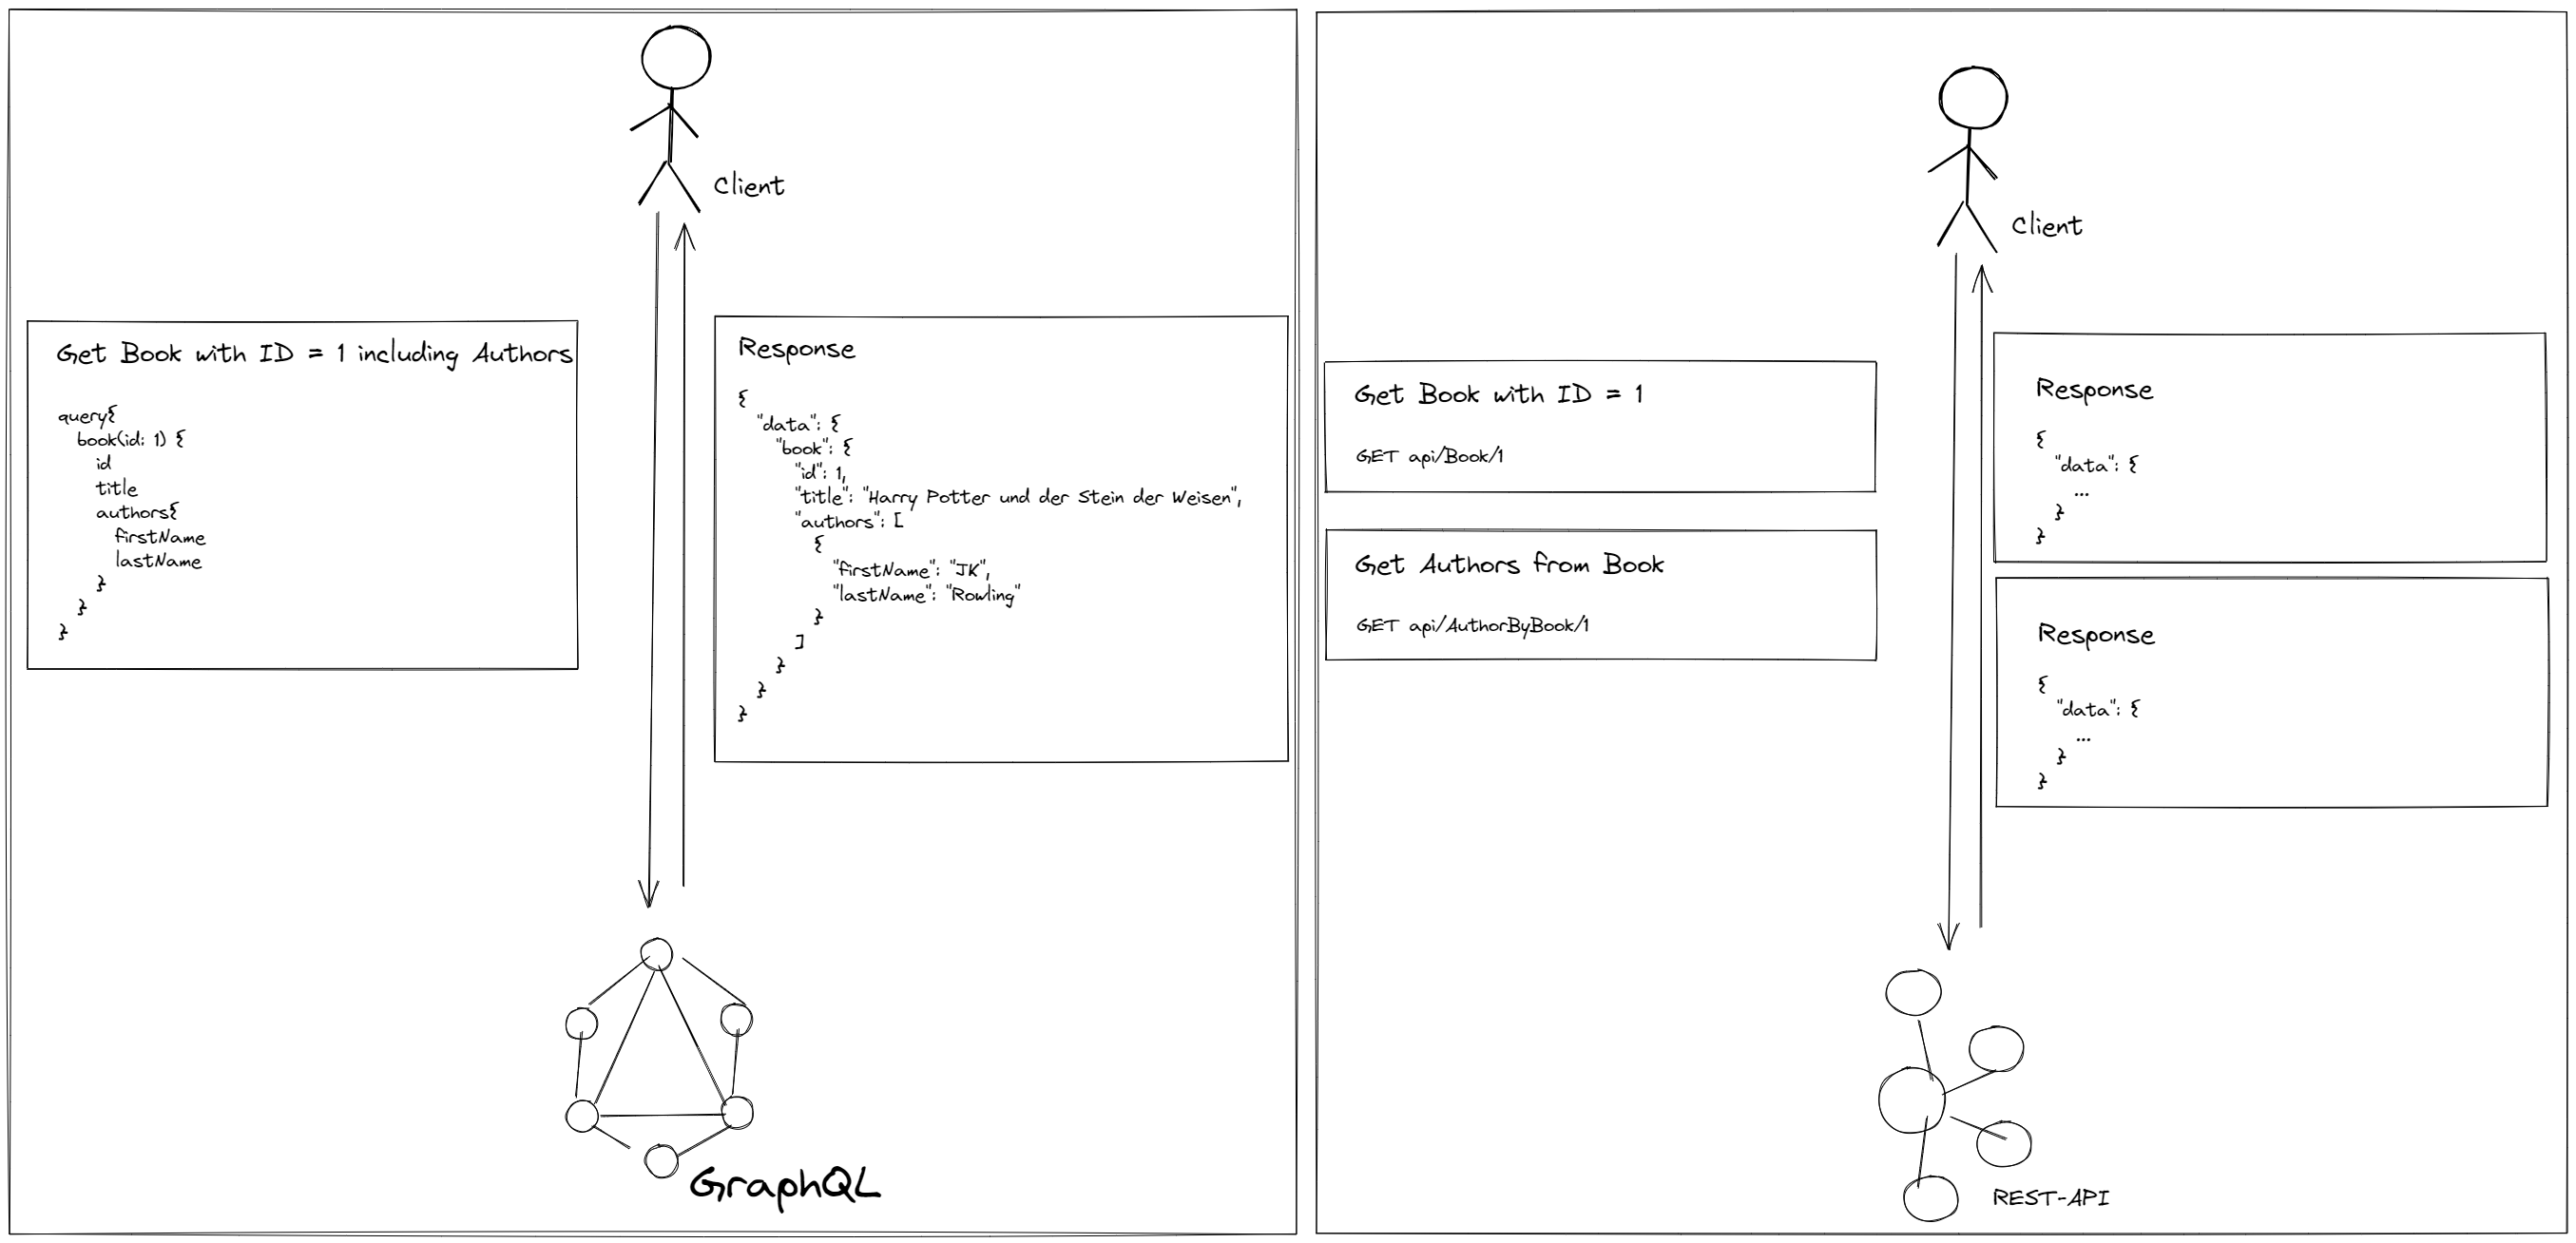
\includegraphics[width=\textwidth]{pics/graphql_rest_request.png}
    \caption{Gegenüberstellung REST-Anfrage / GraphQL-Anfrage}
\end{figure}

In Abbildung 2.1 ist zu sehen, dass ein Client zwei Anfragen an eine REST-API stellen muss, während er bei einem GraphQL-Service nur eine einzige Anfrage benötigt.
Weiters ist zu sehen, dass GraphQL die Daten, welche in der Query abgefragt wurden, genau in dem Schema zurückliefert in dem sie abgefragt wurden.
Dadurch hat GraphQl den Vorteil, dass Antworten auf Anfragen immer vorhersehbar sind \cite[Abs. Basics of a GraphQL API]{rakutenGraphQLVsRest}.

\subsection{Entwurfsprinzipien}
Da GraphQL sprachunabhängig ist, werden in der Spezifikation keine Implementierungsdetails definiert sondern nur Entwurfsprinzipien.
Diese Entwurfsprinzipien werden in den folgenden Abschnitten näher erläutert:

\myparagraph{Produktzentriert}
Die Anforderungen der Clients (Darstellung der Daten) stehen im Mittelpunkt.
GraphQL bietet mit einer Abfragesprache dem Client die Möglichkeit, genau die Daten abzufragen, die er tatsächlich benötigt. Die Hierarchie der
Abfrage wird durch eine Menge ineinander geschachtelter Felder abgebildet \cite[Abs. 1]{graphqlOnline}.

\myparagraph{Hierarchisch}
Eine GraphQL-Anfrage ist hierarchisch strukturiert.
Jede Anfrage ist so geformt wie die Daten die zurückgelifert werden.
Das bedeutet, dass der Client die Daten genau in dem Format erhält, wie diese in der Anfrage spezifiziert wurden.
Das ist ein intuitiver Weg für den Client um seine Datenanforderungen zu definieren \cite[Abs. 1]{graphqlOnline}.

\myparagraph{Strenge Typisierung}
Jeder GraphQL-Service definiert ein anwendungsspezifisches Typ-System.
Anfragen werden im Kontext dieses Typ-Systems ausgeführt.
Mit Tools wie zum Beispiel \textit{GraphiQL} kann man vor Ausführung der Anfrage sicherstellen, dass sie syntaktisch und semantisch korrekt sind \cite[Abs. 1]{graphqlOnline}.

\myparagraph{Benutzerdefinierte Antwort}
Mittels dem Typ-System definiert der GraphQl-Service ein Schema welches er veröffentlicht.
In diesem Schema sind die Zugriffsarten als auch die verwalteten Ressourcen definiert.
Der Client ist zuständig, zu definieren welche Daten er wie abfragen will.
Die meisten anderen Client-Server-Applikationen geben die Form der Daten, welche sie zurückgeben, selbst vor.
Ein GraphQl-Service, retourniert exakt die Daten welche der Client angefordert hat, nicht mehr und nicht weniger \cite[Abs. 1]{graphqlOnline}.

\myparagraph{Introspektion}
Das Typ-System eines GraphQL-Services kann direkt mit der GraphQL-Abfragesprache abgefragt werden. Diese Abfragen werden für die Erstellung von Tools für GraphQL benötigt \cite[Abs. 1]{graphqlOnline}.

\section{GraphQL vs. REST}
\subsection{Endpunkte}
Eine REST-API bietet für jede Ressource verschiedene Endpunkte an um CRUD Operationen für die jeweilige Ressource auszuführen. GraphQL hingegen bietet nur einen
Endpunkt. An diesem kann der Client eine Abfrage mit einer Query oder einer Mutation senden um auf die jeweilige Ressource zuzugreifen.

\subsection{Over-fetching und Under-fetching}
Als Overfetching wird das Laden von zu vielen oder nicht benötigten Daten bezeichnet.
Underfetching bedeutet, dass man mehr Daten benötigt, als der Server dem Client zurückgibt.
Dieses Problem tritt bei REST-APIs auf die viele verschiedene Clients mit Daten versorgen müssen (beispielsweise eine Desktop-Applikation, eine mobile Anwendung und ein Web-Client).
Grundsätzlich wollen alle drei Clients diesselbe Ressourcen abfragen, mit dem Unterschied, dass die mobile Anwendung beispielsweise weniger Daten benötigt.
Die Desktop-Applikation möchte aber alle Daten einer Ressource bekommen, um diese darzustellen.
Eine Lösung dafür wäre beispielsweise, einen Endpunkt für jeden Client zu definieren um die für ihn benötigen Daten zur Verfügung zu stellen.
Dies resultiert aber in einem erhöten Programmieraufwand und damit auch einer höheren Komplexität der Anwendung.
\newline

Dieses Problem kann bei GraphQL nicht auftreten, da der Client in seiner Anfrage genau jene Daten definiert, die er benötigt.

\chapter{GraphQL}
\section{Typ-System}

Das GraphQL-Typ-System wird zur Definition eines Schemas verwendet.
Ein Schema beschreibt einen GraphQL-Service und besteht aus den abrufbaren Ressourcen, ihren Relationen zueinander und ihren Interaktionsmöglichkeiten.


Eine eingehende Anfrage wird durch die im Schema definierte Datenstruktur validiert.
Wenn die in der Anfrage enthaltene Query durch das Typ-System erfolgreich validiert wurde, wird die beinhaltete Operation an die Implementierung weitergeleitet.
Dafür zerlegt GraphQL die übergebene Query und gibt sie an den jeweiligen Resolver weiter. Diese Resolver interagieren mit der Geschäftslogik und füllen die angeforderten Felder mit Daten.
Die kumulierten Ergebnisse werden als Antwort an den Client zurückgeschickt. 
\cite[S. 57-58]{kress2020graphql}
\cite[Abs. Schemadefinition]{graphqlOnline}


\section{Schema-Definitions-Sprache SDL}
Da GraphQL laut Spezifikation in jeder beliebigen Sprache implementierbar sein soll, wird eine sprachunabhängige Basis für die Definition des GraphQL-Graphen benötigt.
Die Grundlage dafür stellt die in der Spezifikation definierte Beschreibungssprache (\textit{SDL}). 
In GraphQL existieren folgende Typ-Definitionen: \textit{Skalar, Interface, Object, Input Object, Enum} und \textit{Union}.
Diese bilden das Rückgrat des Schemas.
Über diese Typen werden in den nachfolgenden Abschnitten genauer behandelt.

\subsection{Skalare}

Ein Datentyp, der nicht mehr weiter vereinfachbar ist, wird wie in anderen Programmiersprachen Skalar-Typ genannt.
Skalar-Typen repräsentieren die Blätter, also die primitiven Werte des GraphQL-Typ-Systems \cite[S. 60]{kress2020graphql}.
GraphQL-Antworten entsprechen der Form eines hierarchisch aufgebauten Baumes.
\newline


Grundsätzlich bestehen die Blätter dieses Baumes aus GraphQL-Skalar-Typen (es ist zudem auch möglich, dass die Blätter aus \textit{Null-Werten} oder \textit{Enum-Typen} bestehen).
\cite[Abs. ScalarTypeDefinition]{graphqlOnline}
GraphQL beinhaltet folgende vordefinierten Skalar-Typen:
\begin{enumerate}
    \item Boolean
    \item Float
    \item Int
    \item String
    \item ID
\end{enumerate}

\begin{JsCode}
    id: Int!
    title: String
\end{JsCode}

Im oben angeführten Codebeispiel werden die Felder \textit{id} und \textit{title} definiert.
Der Name eines Feldes im umgebenden Typ muss dabei eindeutig sein.
Die Deklaration erfolgt mit dem Namen als auch dem Typ des Feldes, welche mit einem Doppelpunkt getrennt sind.
Das Feld \textit{id} wird dabei mit einem Rufzeichen (!) als \textit{not null} deklariert.

\myparagraph{Benutzerdefinierte Skalare}


In den meisten sprachspezifischen Implementierungen ist es möglich, eigene Skalar-Typen zu definieren. Diese werden verwendet, um beispielsweise verschiedene Datumsformate darzustellen.

\subsection{Enum}

Enum-Typen stellen wie Skalare die Blätter des Typ-Baums dar.
Ein Enum-Feld hält ein spezifisches Element aus einer Menge von möglichen Werten
\cite[Abs. 3.9]{graphqlOnline}
\cite[S. 60-61]{kress2020graphql}.

\begin{JsCode}
enum Category {
    Fantasy
    Adventure
    Mystery
    Thriller
    Romance
}
\end{JsCode}

In diesem Beispiel wurde ein Enum \textit{Category} definiert.
Es gilt zu beachten, dass dieser Typ mit dem Schlüsselwort \textit{enum} definiert werden muss.

\subsection{Objekt}
Wie bereits erwähnt bestehen die Blätter des Baumes in GraphQL aus den Skalar-Typen.
Die Knoten wiederum werden von Objekt-Typen definiert.
Diese Objekte halten eine Liste von Feldern die einen bestimmten Wert lieferen.
Jedes Feld kann entweder ein Skalar, ein Enum, ein Objekt oder ein Interface sein.
Laut Spezifikation, sollten Objekte als eine Menge von geordneten Schlüssel-Wert-Paaren serialisiert werden.
Wobei der Name des Feldes der Schlüssel ist und das Ergebnis der Evaluierung des jeweiligen Feldes den Wert abbildet.
Um einen Objekt-Typ zu definieren muss das Schlüsselwort \textit{type} verwendet werden
\cite[Abs. 3.6]{graphqlOnline}.

\begin{JsCode}
type Book {
    id: Int!
    title: String
    authors: [Author]
}
    
type Author {
    id: Int!
    firstName: String
    lastName: String
    books: [Book]
}
\end{JsCode}

Im oben angeführten Schemaausschnitt werden die beiden Objekte \textit{Author} und \textit{Book} definiert.
Um einen Objekttypen zu definieren wird das Schlüsselwort \textit{type} verwendet.

Das Objekt Book wird dabei mit den Feldern \textit{id, title} und \textit{authors} definiert.
Das Objekt Author erhält die Felder \textit{id, firstName, lastName} und \textit{books}.

Die Felder \textit{id, title, firstName} und \textit{lastName} sind dabei skalare Felder und bilden dabei Blätter des Baumes.
Da zwischen den Objekten Author und Book eine n:m Beziehung besteht, halten beide Objekte eine Liste des jeweils anderen Objekt-Typs.
Listen werden in der SDL wie im obigen Beispiel ersichtlich mit eckigen Klammern definiert.

\subsection{Interface}

Interfaces sind abstrakte Typen welche eine Liste an Feldern definieren.
GraphQL-Interfaces repräsentieren eine Liste von Felder und deren Argumente.
Objekte und Interfaces können ein Interface implementieren, dazu muss der Typ, welcher das Interface definieren will, alle Felder des zu implementierenden Interfaces definieren.
\newline
\cite[Abs. 3.7]{graphqlOnline}
Felder eines Interfaces sind an dieselben Regeln wie ein Objekt gebunden.
Der Typ eines Feldes kann entweder ein Skalar, Enum, Interface oder Union sein.
Zudem ist es möglich, dass ein Typ mehrere Interfaces implementiert.
\cite[S.65-66]{kress2020graphql}
\newline


Im folgenden Codebeispiel wird die Definition eines Interfaces veranschaulicht:

\begin{JsCode}
interface Person {
    firstName: String
    lastName: String
}

type Author implements Person {
    id: Int!
    firstName: String
    lastName: String
    books: [Book]
}
\end{JsCode}

Jedes Interface benötigt eine spezifische Implementierung, im angeführen Beispiel implementiert \textit{Author} das Interface \textit{Person}.
Author muss dabei alle Felder von \textit{Person} zur Verfügung stellen.

\subsection{Input-Objekt}
Ein Input-Objekt ist ein spezieller Objekt-Typ. Ein Input-Objekt hält genauso wie ein Objekt-Typ skalare Felder, Enumerationen oder Referenzen.
Diese referenzierten Objekt-Typen müssen aber ebenso Input-Objekte sein.
Eine Mischung der Objekt-Typen ist laut Spezifikation nicht erlaubt.
Ein Input-Objekt unterscheidet sich zu einem Objekt-Typ nur durch das Schlüsselwort \textit{input} anstatt von \textit{type}.
Weiters können die Felder eines Input-Objekts keine Argumente beinhalten.
\newline


Im folgenden Beispiel wird ein Input-Objekt für ein Buch realisert:
\begin{JsCode}
input AuthorCreateInput {
  firstName: String
  lastName: String
  books: [Int!]
}
\end{JsCode}

\subsection{Fragmentierung}\label{sec:Bezeichnung}
Fragmente helfen dabei den Text von Abfragen zu reduzieren indem sie oft gebrauchte Abfragen von Feldern kapseln.
Weiters können Fragmente nur für Objekt-Typen, Interfaces und Union-Typen definiert werden.
Fragmente müssen dabei den Objekt-Typen für den sie gelten mit dem Schlüsselwort  \textit{on} angeben.
Inline-Fragmente müssen nicht mit dem Schlüsselwort \textit{fragment} definiert werden.
Sie können mit dem Spread-Operator direkt in der Abfrage definiert werden \cite[Abs. 2.8 -  2.8.1]{graphqlOnline}.
Fragmente liefern nur dann Daten zurück wenn der Objekt-Typ der sie anfordert auch wirklich dem Typen des Fragments entspricht.

Im folgenden Beispiel wird ein Fragment für den Objekt-Typ Author definiert, weiters wird die Verwendung in einer Query veranschaulicht:
\begin{JsCode}
fragment authorFragment on Author {
    firstName
    lastName
}

\end{JsCode}


Im nachfolgenden Beispiel wird die Nutzung eines Inline-Fragments in einer Query veranschaulicht:
\begin{JsCode}
query{
    books{
        title
        on Author{
            firstName
            lastName
        }
    }
}
\end{JsCode}

\subsection{Union}
Union-Typen fügen mehrere Objekte zu einer Gruppe zusammen.
Diese Typen sind sehr nützlich, wenn beispielsweise eine Query zwei unterschiedliche Objekt-Typen zurückgeben kann, diese aber nicht diesselben Felder besitzen.
In dieser Query können dann mithilfe von Inline-Fragmenten (siehe \ref{sec:Bezeichnung}) die spezifischen Felder abgefragt werden.

\begin{JsCode}
union SearchResult = Author | Buch
\end{JsCode}

\subsection{Direktive}
Direktiven bieten die Möglichkeit die Struktur, des durch eine Query angefragtes Ergebnis zu beeinflussen.
Mittels einer Annotation direkt an einem Feld oder einer Objekt-Relation
Mit Direktiven ist es möglich mittels Annotationen, direkt an einem Feld oder einem Objekt-Typen, dasselbige entsprechend einer Eingabe zu beeinflussen.
GraphQL bietet dafür standardmäßig zwei Arten von Strukturmanipulationen: \textit{@include} und \textit{@skip}, es ist aber auch möglich serverseitig zusätzliche Direktiven zu implementieren.
Mittels diesen Direktiven lassen sich Objekt-Typen oder Felder inkludieren oder überspringen.
Für die auszuwertende Direktive muss dabei in der Query ein \textit{Boolean} mitübergeben werden.

Im folgenden Beispiel wird eine Direktive gezeigt welche standardmäßig das Feld \textit{id} ignoriert.

\begin{JsCode}
query {
    authors($withoutId: Boolean = false){
        id @include(if: $withoutId)
        firstName
        lastName
    }
}
\end{JsCode}


\section{Schema}
Im Schema welches mittels der \textit{SDL} definiert wird, werden alle Objekt-Typen des GraphQL-Services definiert.
Durch das Schema werden die verwalteten Entitäten durch Objekt-Typen definiert.
Weiters werden auch die vom GraphQL zur Verfügung gestellten Interfaces, Unions, Fragments, Direktiven, Enums und Input-Typen definiert.
Wenn man die im Schema definierten Objekt-Typen als Baumstruktur betrachtet so sind die referenzierten Objekt-Typen Verzweigungen des Baumes.
Die Blätter am Ende des Baumes enthalten die eigentlichen Daten.
Die Astverzweigungen sind von besonderer Bedeutung, denn sie beinhalten die Referenzen zu den anderen Objekt-Typen.
\cite[S.60]{kress2020graphql}

Weiters dürfen die im Schema definierte Namen nicht mit doppeltem Unterstrich beginnen.
Diese sind für das GraphQL Introspektionsystem reserviert.
\cite[Abs. 3.3]{graphqlOnline}

\section{Wurzel Operationen}
Das Schema definiert die Wurzelknoten der Eingangspunkte der Operationen (Query, Mutation und Subscription) die es unterstützt.
Das Schema definiert dadurch den Eingangspunkt dieser Operationen im Typ System.
Diese Wurzeloperationen sind spezielle Objekt-Typen.
Um ein korrektes Schema zu erstellen muss beachtet werden, dass die Typen und Direktiven eindeutig über ihren Namen identifizierbar sind.
Query muss aber zwingend definiert werden. Mutations und Subscriptions sind optional und werden, wenn sie nicht explizit definiert werden, nicht unterstützt.
Desweiteren müssen die Objekt-Typen der Wurzel-Operationen unterscheiden und dürfen nicht diesselben sein. 
\newline


\section{Schema Definition}

% \begin{figure}[H]
%     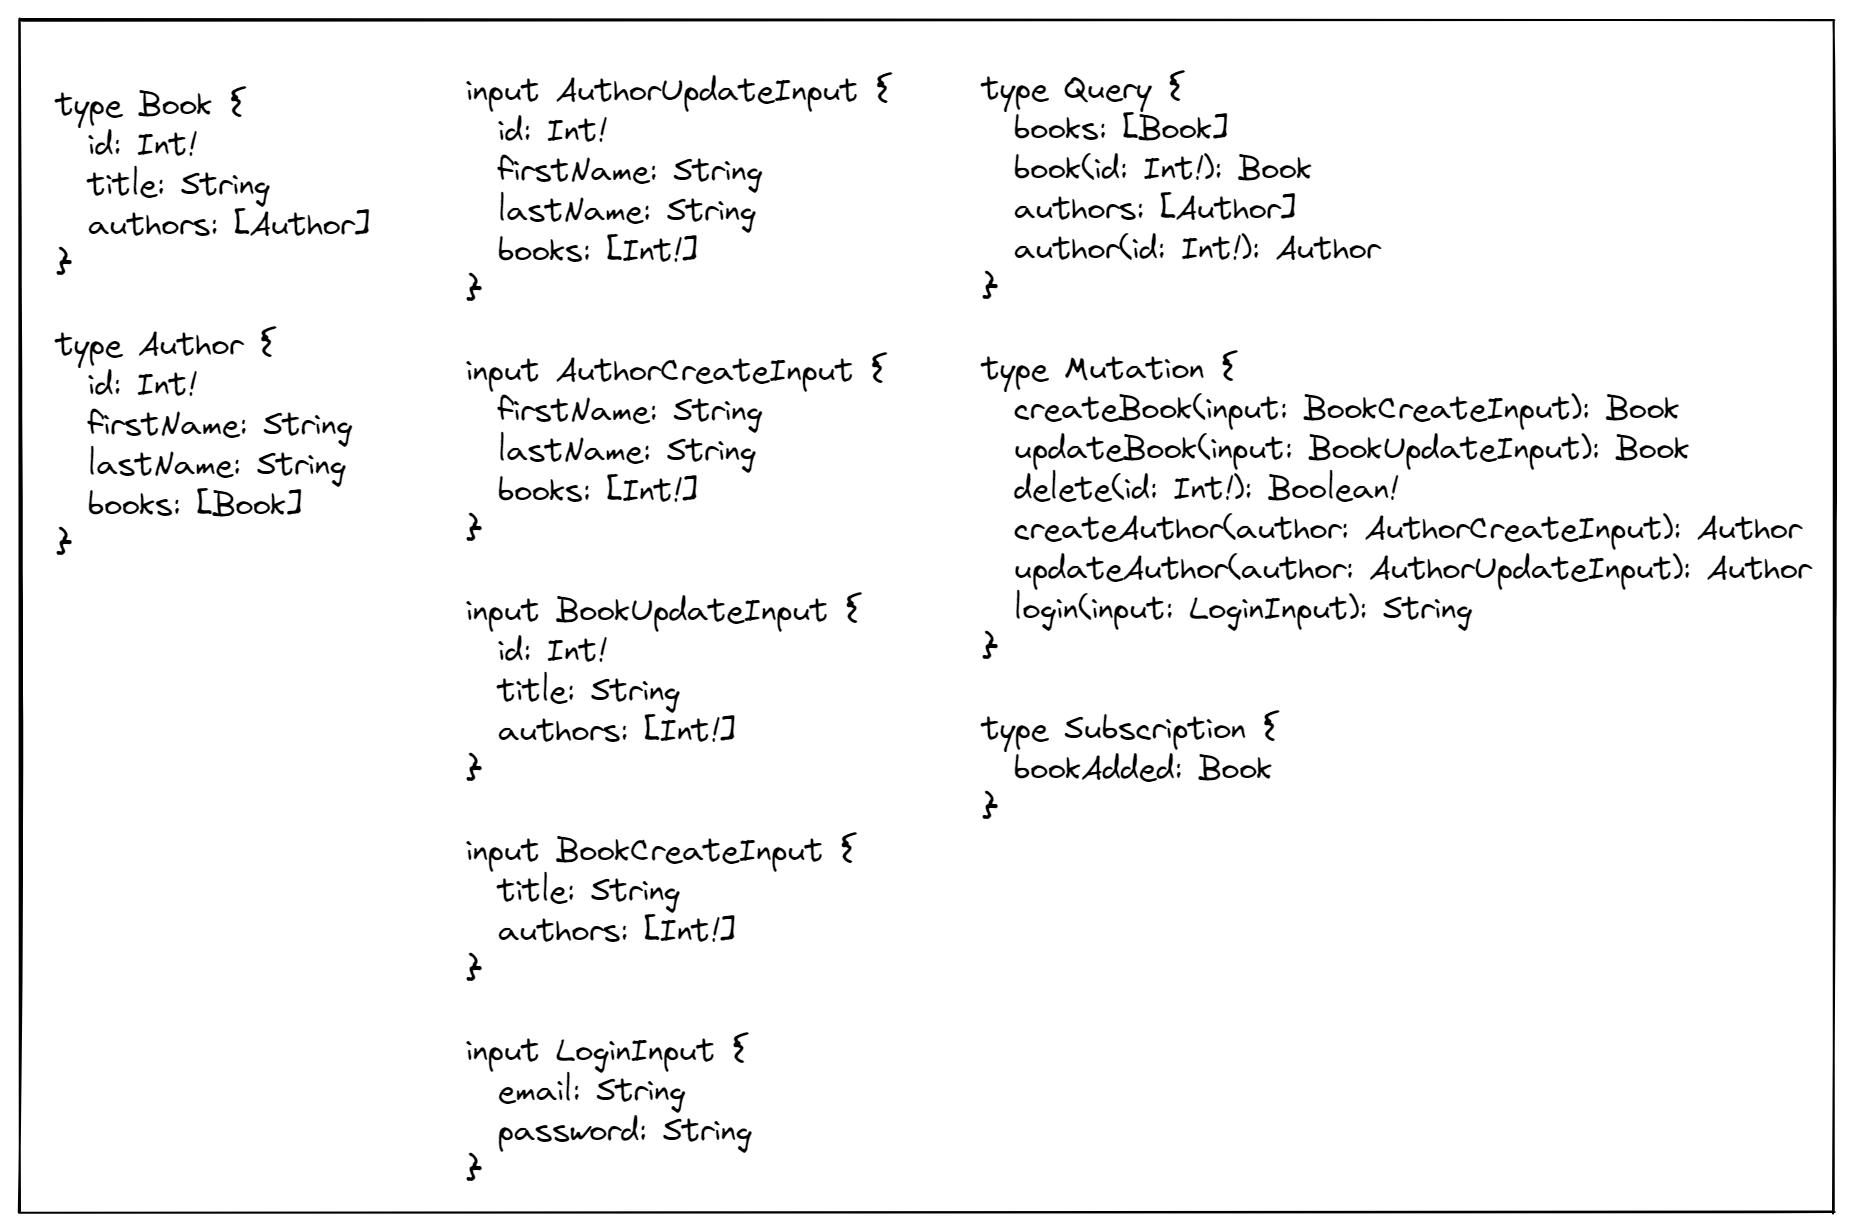
\includegraphics[width=\textwidth]{pics/schema.png}
%     \caption{Schemadefinition}
% \end{figure}

\begin{JsCode}
type Book {
    id: Int!
    title: String
    authors: [Author]
}
    
type Author {
    id: Int!
    firstName: String
    lastName: String
    books: [Book]
}
    
type Review {
    userId: Int!
    user: User!
    bookId: Int!
    book: Book!
    rating: Int!
    id: Int!
}
    
type User {
    firstName: String!
    lastName: String!
    email: String!
    roles: [Role!]!
    reviews: [Review!]!
    id: Int!
}
    
input AuthorUpdateInput {
    id: Int!
    firstName: String
    lastName: String
    books: [Int!]
}
    
input AuthorCreateInput {
    firstName: String
    lastName: String
    books: [Int!]
}
    
input BookUpdateInput {
    id: Int!
    title: String
    authors: [Int!]
}
    
input BookCreateInput {
    title: String
    authors: [Int!]
}
    
input LoginInput {
    email: String
    password: String
}
    
input ReviewUpdateInput {
    id: Int!
    userId: Int!
    bookId: Int!
    rating: Int!
}
    
input ReviewCreateInput {
    userId: Int!
    bookId: Int!
    rating: Int!
}
    
input LoginDataInput {
    email: String!
    password: String!
}
    
input UserInput {
    firstName: String!
    lastName: String!
    email: String!
    password: String!
    id: Int!
}
    
type Query {
    books(where: BookFilterInput, order: [BookSortInput!]): [Book!]!
    book(where: BookFilterInput, order: [BookSortInput!]): Book
    authors(where: AuthorFilterInput, order: [AuthorSortInput!]): [Author!]!
    author(where: AuthorFilterInput, order: [AuthorSortInput!]): Author
    reviews(where: ReviewFilterInput, order: [ReviewSortInput!]): [Review!]!
    author(where: ReviewFilterInput, order: [ReviewSortInput!]): Review
}
    
type Mutation {
    register(input: UserInput): User
    login(input: LoginDataInput): String
    createBook(input: BookCreateInput!): Book!
    updateBook(input: BookUpdateInput!): Book!
    createAuthor(input: AuthorCreateInput!): Author!
    updateAuthor(input: AuthorUpdateInput!): Author!
    createReview(input: ReviewCreateInput!): Review!
    updateReview(input: ReviewUpdateInput!): Review!
}
    
type Subscription {
    bookAdded: Book
}
\end{JsCode}

In Abbildung 3.1 ist eine Schemadefinition zu sehen welche Objekt-Typen, Input-Typen und die Wurzeloperationen beinhaltet.

\section{Zugriff auf den GraphQL-Service}
GraphQL liefert keine Spezifikation über die Netzwerkschicht, sondern lediglich eine Empfehlung \textit{HTTP} zu verwenden.
Im Gegensatz zu \textit{REST-APIs} beschränkt sich GraphQL auf lediglich zwei HTTP-Methoden: GET und POST.
Deswegen ist die Gestaltung und Bennung der Endpunkte nicht so relevant wie bei REST-APIs.
\newline

Der Unterschied, ob ein Client mittels GET oder POST-Anfrage auf den Service zugreift, besteht darin, dass mittels GET-Anfrage nur lesende Zugriffe möglich sind.
Also können mit GET-Anfragen nur Querys aber keine Mutations umgesetzt werden.
Desweiteren müsste man jene Query, welche zum Abfragen der Daten verwendet werden sollte, als URL-Parameter übergeben.
Somit gilt es auch zu beachten die Sonderzeichen der Query in \textit{ASCII} umzuwandeln.
\newline

Wenn man nun also mittels GET-Anfrage eine Query an den GraphQL-Service schickt, resultiert es in dem Nachteil, dass man eine wesentlich schlechtere Übersicht hat. 
Denn die URL-Encodierung verkompliziert die Anfrage und sorgt für Einschränkungen in der Lesbarkeit.
Etwaig benötigte Variablen müssten auf dieselbe Art und Weise der Anfrage hinzugefügt werden.
Problematischer ist dabei aber jedoch, dass einige Browser eine Maximallänge für URIs definiert haben.
Somit können komplexe Querys nicht funktional sicher über GET-Anfragen abgebildet werden.
\newline

Aus diesem Grund ist es Standard, dass in GraphQL alle Anfragen per POST-Anfrage abgewickelt werden.
Diese werden an den einzigen, nach außen freigegebenen Endpunkt gerichtet.
Da für die Anfragen die POST-Methode verwendet wird, können im Body beliebig viele und komplexe Querys an den Service übergeben werden.
\newline

Grundsätzlich besteht eine Anfrage an den GraphQL-Service aus der eigentlichen Query und zwei optionalen Parametern: Variablen und der Name der Operation.


% Um schreibend oder lesend auf den GraphQL-Service zugreifen zu können muss an den bereitgestellten Endpunkt eine POST-Anfrage mit einer Query geschickt werden.
% Diese Query ist mittels der \textit{GraphQL Query Language GQL} definiert.
% Eine Anfrage welche eine Query beinhaltet, hat zusätzlich noch zwei optionale Parameter: \textit{variables} und \textit{operationName}.
% Der Name einer Operation wird jedoch nur benötigt wenn mehrere Operationen in der Query auszuführen sind.
% graphql.org/learn/serving-over-http

% Gress Seite 82-83

\section{Querys}

Querys bieten den Clients die Möglichkeit lesend auf die Objekte, welche vom GraphQL-Service verwaltet werden, zuzugreifen.
GraphQL erlaubt es dem Client genau die Daten abzufragen welche er benötigt.
Um auf eine Ressource zuzugreifen wird ein POST-Request an den Wurzelknoten der GraphQL-Applikation geschickt.
Dieser POST-Request enthält ein in der \textit{GraphQL Query Language} definiertes Objekt.
In diesem Objekt werden die auszuführenden Funktionen definiert und welche Felder davon an den Client zu retournieren sind.
Das Ergebnis hat genau jenes Format welches in der Anfrage vom Client definiert wurde.
\cite[S.40-41]{kress2020graphql}

Da GraphQL mit einem Graphenschema arbeitet, welche auf den Beziehungen der Knoten zueinander basiert, ist es möglich diese Relationen zu nutzen um Daten über mehrere Objekte hinweg zu sammeln.
\newline


In der folgenden Abbildung ist eine verschachtelte Query zu sehen, welche alle Bücher mit den dazugehörigen Autoren anfordert.

\begin{figure}[H]
    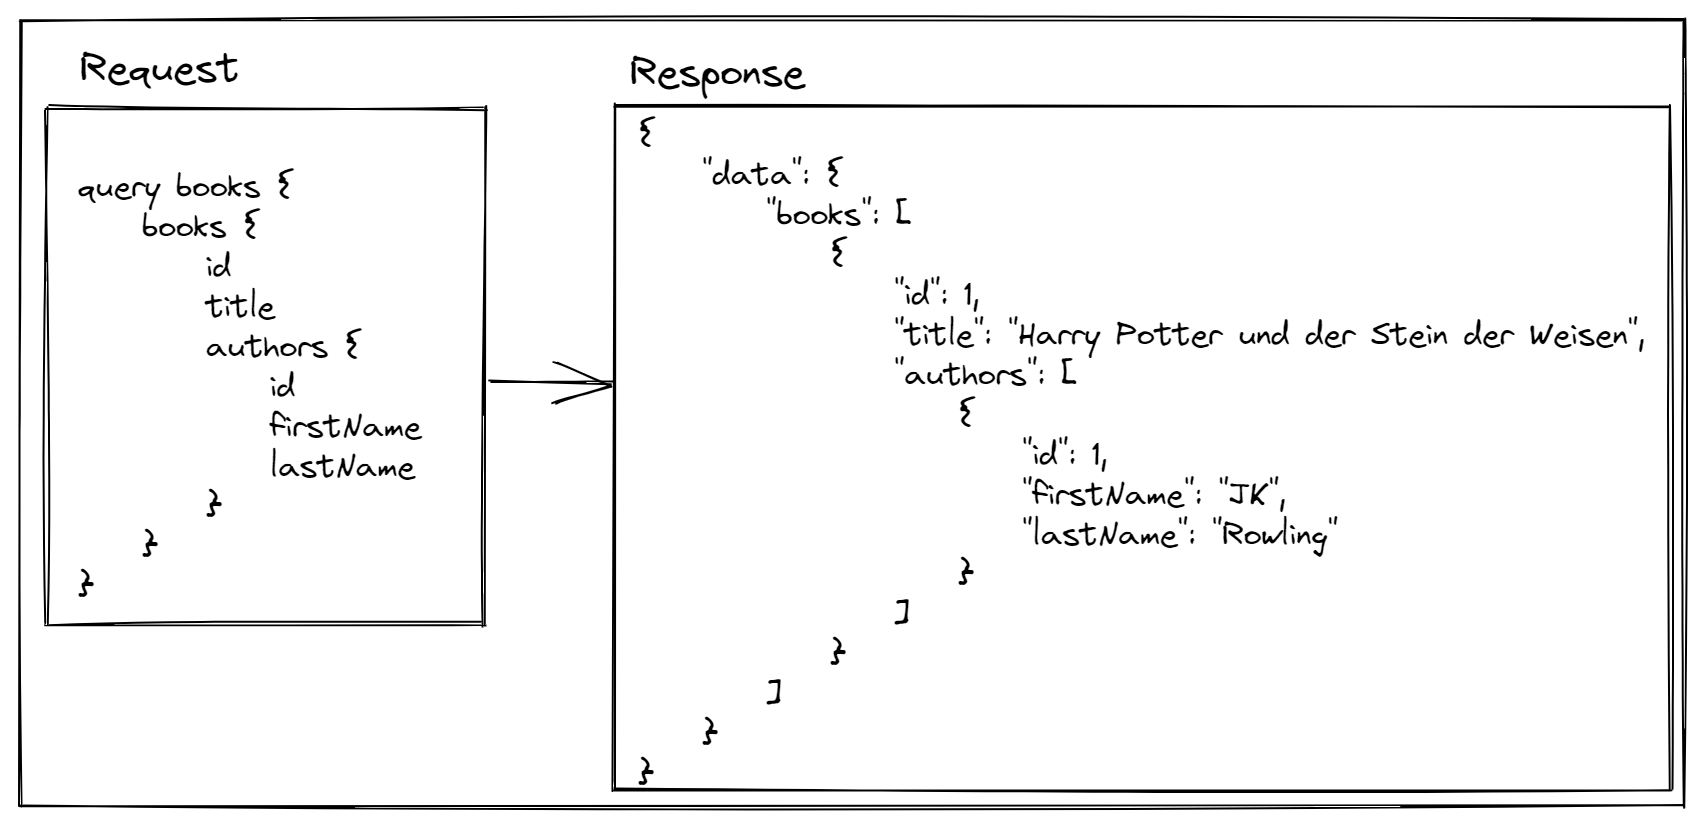
\includegraphics[width=\textwidth]{pics/query_book_with_result.png}
    \caption{Anfrage aller Bücher mit zugehörigen Autoren.}
\end{figure}

\section{Parameter}
Felder können zusätzlich noch Parameter halten.
Diese Parameter können den Rückgabewert des Feldes ändern um das Feld noch flexibler zu machen.
\newline

\begin{JsCode}
enum Currency {
    EUR
    USD
    GBP
}

type Book {
    id: Int!
    title: String
    authors: [Author]
    price: (unit: Currency = EUR): Float
}
\end{JsCode}

Im oben stehenden Code Beispiel wurde der Objekt-Typ Book um ein Feld \textit{price} erweitert.
Bei einer Query auf das Feld price des Objekts Book kann ein Argument unit mitgegeben werden um den tatsächlichen Verkaufswert in der richtigen Währung zu bestimmen.
Dabei wurde ebenfalls ein Standardwert definiert um unit nicht zwingend als Parameter übergeben zu müssen.
\cite[S.62]{kress2020graphql}


\subsection{Variablen}
Mit Parametern ist es möglich zusätzliche Daten für spezielle Operationen an den GraphQL-Service zu schicken.
Diese können aber nur statisch in die Query eingetragen werden.
Deswegen kann eine GraphQL Operation zudem mit Variablen erweitert werden.
Dadurch hat man verstärkt die Möglichkeit Funktionen wiederzuverwenden.
Variablen müssen am Anfang einer Operation definiert werden und befinden sich während der Ausführung im Lebensraum der Operation.
Diese Variablen werden unter anderem für die Filterung der angeforderten Objekte verwendet.
\cite[Abs. 5.8]{graphqlOnline}
\newline

In der folgenden Abbildung ist eine Anfrage zu sehen welche das Buch mit der \textit{id = 1} anfordert. Dabei wird die id als Variable übergeben.

\begin{figure}[H]
    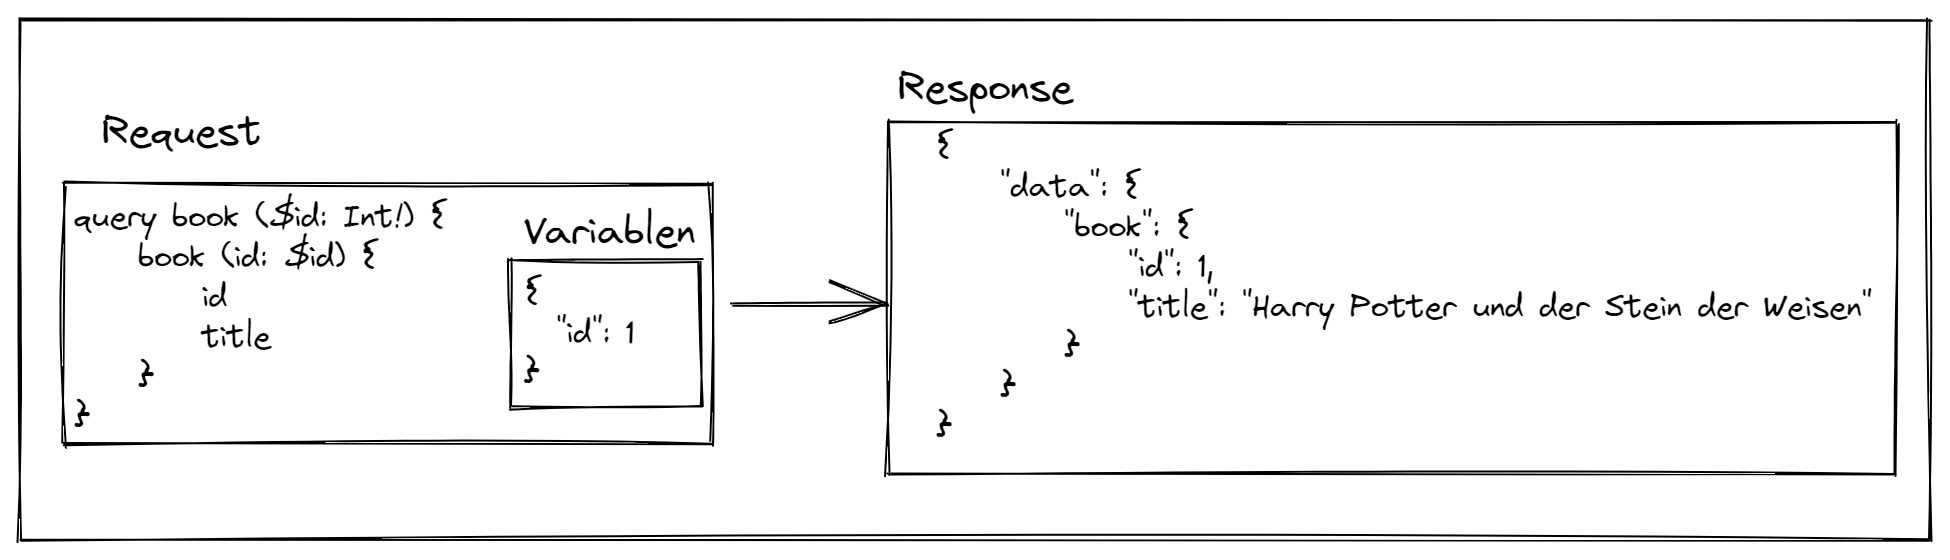
\includegraphics[width=\textwidth]{pics/book_request_with_parameter.png}
    \caption{Anfrage aller Bücher mit zugehörigen Autoren unter Verwendung einer Variable.}
\end{figure}

% \subsection{Aliase}
% In GraphQL-Queries ist es möglich, dass mehrere miteinander in Konflikt stehende Parameter übergeben werden.
% Um diesem Problem vorzuwirken besteht die Möglichkeit mit \textit{Aliases} zu arbeiten.
% Mit ihnen ist es möglich die unterschiedlichen Resultate dieser in Konflikt stehenden Argumente zu benennen und damit zu unterscheiden.
% % Kress 46
% \cite[S. 46]{kress2020graphql}

\section{Mutationen}
APIs benötigen neben dem lesenden Zugriff auf Daten auch einen schreibenden.
Dieser wird in GraphQL mittels Mutationen umgesetzt.
Mutationen kapseln die Implementierungen der Datenbankzugriffsschicht in ein Interface welches die Möglichkeiten zur Manipulation der Daten vorgibt.
Manipulierende Anfragen können Daten dadurch nur auf jene Art und Weise ändern, wie es in der Applikation vorgesehen ist.
% Kress 54
\cite[S. 54]{kress2020graphql}


% Mutationen ermöglichen es die Zugriffe 
% Sie werden in der Schemasprache (anderer Begriff ??? -> GDL etc)  mit dem Schlüsselwort mutation definiert.


\section{Subscriptions}
% Durch diese spezielle Form der Querys ist es möglich Daten in Echtzeit zu folgen und Updates direkt vom Server zu erhalten wenn gewisse Events ausgelöst wurden.
% Diese Events werden meist durch das Erzeugen, ändern oder löschen von Daten ausgelöst.

Subscriptions sind eine spezielle Form von Query.
Sie werden verwendet um den Client vom Server aus über Events zu notifizieren.
Notifizierungen werden in der Regel durch Hinzufügen, Ändern oder Löschen von Datenbankobjekten ausgelöst.
Subscriptions halten eine aktive Verbindung zwischen dem GraphQL-Service und dem Client offen.
Diese Verbindung wird meistens mit WebSockets umgesetzt.
Mit Subscriptions ist es zum Beispiel möglich den aktuellen Bestand von Produkten immer direkt am Client verfügbar zu haben.
Mit dieser Information kann auf der Client-Seite gewährleistet werden, dass ein Benutzer nur ein Produkt kaufen kann, welches noch verügbar ist.
\newline

% Weil sich der Server die Clients merken muss, ändert sich der Status des Systems von einem \textit{statless} zu einem \textit{stateful} API.
% Dadurch wird wiederum die Komplexität des Systems erhöht und die Skalierbarkeit erschwert.

\section{Bekannte Probleme}

\subsection{Authentifizierung, Autorisierung und Rollenmanagement}

\subsection{1 + n Problem}

\subsection{Fehlermanagement}

\subsection{Pagination}

\subsection{Caching}


\chapter{Entwicklung eines GraphQL-Service in .NET mit HotChocolate}
In diesem Kapitel wird die Entwicklung des Prototypen beschrieben.
Der Prototyp ist ein GraphQL-Service welcher mit .NET 6 und der Zuhilfenahme der Bibilothek HotChocolate entwickelt wurde.
Desweiteren wird auf die von HotChocolate bereitgestellten Entwicklerhilfsmittel eingegangen.


\section{Anwendungsszenario}
% Der Anwendungsfall des Prototypen lässt sich wie folgt beschreiben:
% Da die Verwaltungen von Büchern und dazugehörige Autoren und Bewertungen ein aufwändiges Verfahren ist soll 
Die Auswahl eines neuen Buches ist oftmals ein sehr schwieriges Unterfangen.
Bei der Entscheidungsfindung helfen oft Bewertungen von Lesern die das jeweilige Buch schon gelesen haben.
Demnach soll eine Bücher-Bewertungsplattform geschaffen werden.
Diese Plattform ermöglicht es Benutzern Bücher zu bewerten und Informationen über Bücher, Autoren oder Bewertungen einzusehen.
% Benutzer, mit mehr Rechten als reinen Benutzerrechen, haben zudem die Möglichkeit die zusätzlich benötigten Entitäten 
Weiters sollen Benutzer in der Lage sein sich im System zu registrieren und anzumelden.
Angemeldete Benutzer haben, je nach ihren Benutzerrollen, Möglichkeiten im System verwaltete Entitäten zu Erstellen, zu Bearbeiten oder zu Löschen.

\section{HotChocolate}
Für die Implementierung des GraphQL-Service wurde das Framework HotChocolate herangezogen.
Zusätzlich zum HotChocoalte Framework gibt es noch das .NET GraphQL Framework.
Der Prototyp wurde aufgrund der steigenden Beliebtheit und Aktivät der Community des HotChocolate Frameworks mit eben jenem Framework umgesetzt.

\myparagraph{Was ist HotChocolate}
HotChoclate ist ein Open-Source Framework zur Implementierung eines GraphQL-Services.
Es ist konform laut den GraphQL-Spezifikationen implementiert und bietet somit Kompatibilität gegenüber allen anderen GraphQL konform umgesetzten Clients wie zum Beispiel den Apollo Client.
Ein großer Teil der Komplexität einen GraphQL-Service zu schreiben ist dabei die Entwicklung des Schemas.
HotChoclate kümmert sich dabei um die Generierung des Schemas zur Laufzeit und entfernt somit einen großen Teil dieser Komplexität vom Entwickler.

\myparagraph{Schema Erstellung in HotChocolate}
Um das Schema in HotChocolate zu definieren gibt es 3 Varianten: \textit{Pure-Code-First}, \textit{Code-First} und \textit{Schema-First}.
Schema-First nimmt dabei ein bereits bestehendes Schema und fügt es dem Service zu.
Pure-Code-First verwendet Annotationen um das Schema zu definieren.
Code-First verwendet eine Fluent-API, mit allen Varianten erhält man dieselben Ergebnisse im Schema, wobei Code-First dabei das fein granularste Ergebnis liefert.


\section{Architektur}
Der Prototyp wurde mit der für REST-APIs üblichen Drei-Schicht-Architektur umgesetzt.
Die Geschäftslogikschicht und Datenbankzugriffsschicht wurden dabei so entwickelt, dass sie eigentlichen Implementierungen je nach Bedarf einfach ausgetauscht werden können.
Auf die Geschäftslogik wird in den Unterkapiteln Query, Mutation und Subscription näher eingegangen. Die Datenbankzugriffsschicht wird im Kapitel Entity Framework näher erläutert.
\newline

\begin{figure}[H]
    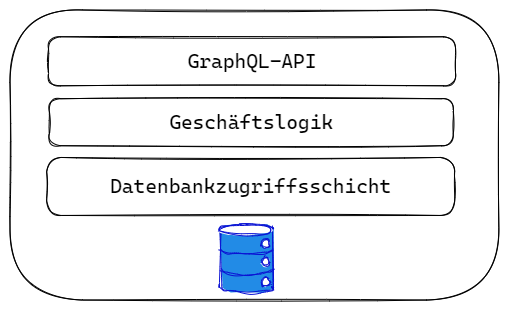
\includegraphics[width=\textwidth]{pics/architecture.png}
    \caption{Drei-Schicht-Architektur}
\end{figure}

Die hier abgebildete Architektur dient zur Veranschaulichung, die gezeigten Schichten werden in den folgenden Unterkapiteln genauer erklärt.

\subsection{API:}
Die API bildet die einzige Schnittstelle des Systems zur Außenwelt.
Sie wird mittels dem GraphQL-Schema abgebildet.
Dieses Schema definiert wie im GraphQL-Kapitel bereits erwähnt die verfügbaren Typen (Objekt-Typen, Input-Typen, ...) als auch die lesenden und schreibenden Zugriffe die der Service zur Verfügung stellt.

Bevor man sich als Entwickler an die Definition des Schemas heranwagt, sollte man zuallererst die Use-Cases, welche der Service zu erfüllen hat definieren.
Die Use-Cases, welcher der Prototyp zu erfüllen hat, sind in der folgenden Abbildung anschaulich dargestellt:

\begin{figure}[H]
    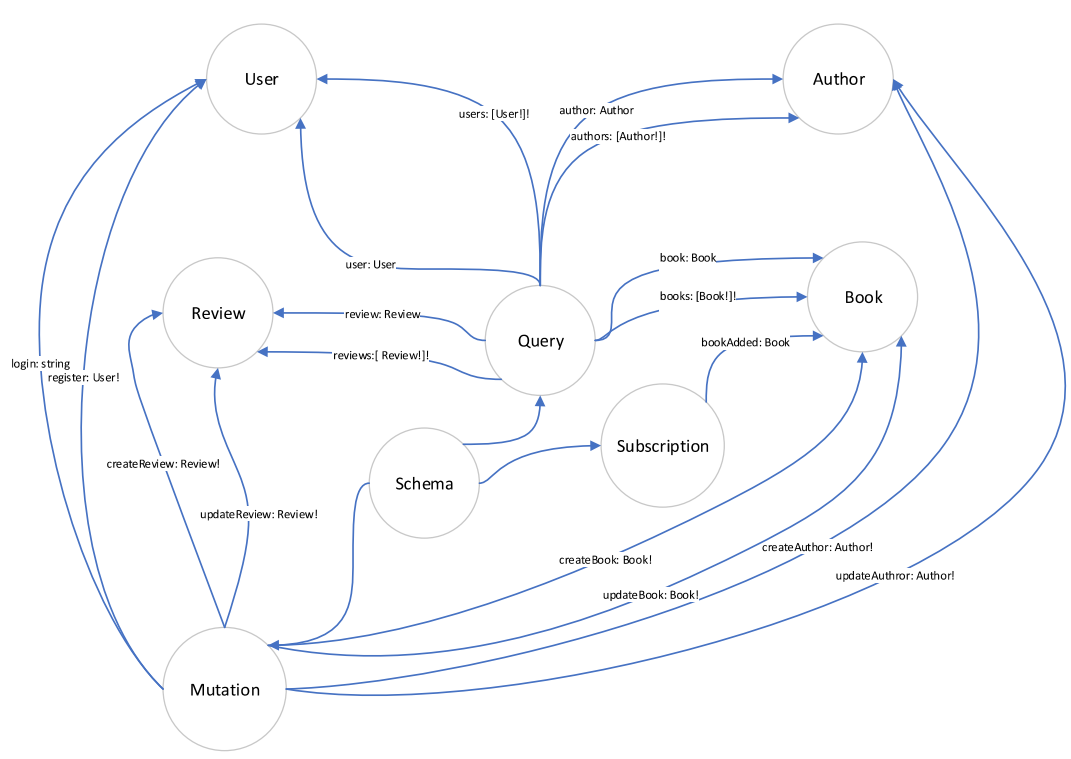
\includegraphics[width=\textwidth]{pics/graph_usecases.png}
    \caption{Use-Cases des Service.}
\end{figure}

In der Grafik ist das Schema anschaulich verdeutlicht.
Es zeigt das Schema und die Definierung der Wurzeloperationen für Query, Mutation und Subscription.
Weiters zeigt es die Operationen welche von den Queries, Mutations und Subscriptions auf die Entitäten abgebildet werden können.

Die Relationen zwischen den Entitäten sind im folgenden ER-Diagram dargestellt:
\begin{figure}[H]
    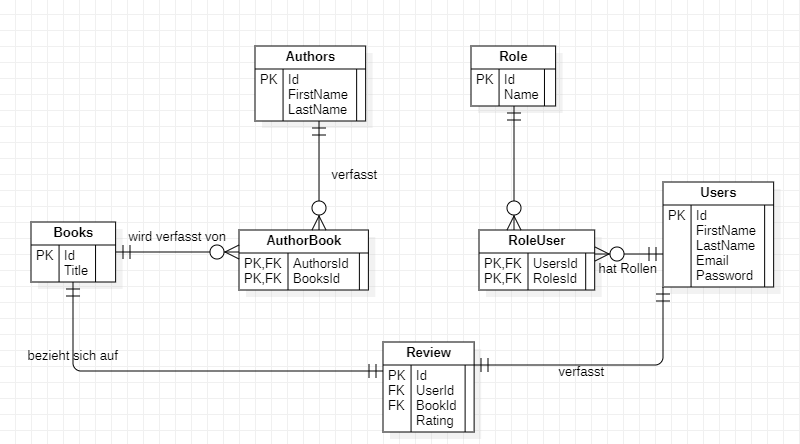
\includegraphics[width=\textwidth]{pics/ER-Diagram.png}
    \caption{Datenbankschema}
\end{figure}

\myparagraph{Definierung des Schemas mit HotChocolate}
% Die API die einzige Schnittstelle des Systems zur Außenwelt.
% \newline

\subsection{Geschäftslogik:}
Die Geschäftslogik bildet dabei die Logik der Server-Applikation ab.

GraphQL an sich ist gegliedert, oben ist die API darunter die Resolver, API selber (Schema) hat kein Wissen über das holen / schreiben der Daten sondern liefert nur Struktur.
Resolver kümmern sich um den Rest.
% \newline

\subsection{Datenbankzugriff:}
Die darunterliegende Datenbankzugriffsschicht ermöglicht, den darüberliegenden Schichten, CRUD-Operationen auf die angeforderten Daten auszuführen.
% \newline


\section{Hot Chocolate}
Der GraphQL-Service wurde mit dem Framework \textit{Hot Chocolate} umgesetzt.
Bei Hot Chocolate handelt es sich um einen Open Source GraphQL-Server welche 

WICHTIG --> Dependency Injection %TODO
PooledDB Context


\subsection{Entwurf Schema}

\section{Entity Framework}
Die Datenbankzugriffsschicht wurde mit dem \textit{Entity Framework} umgesetzt.
Das Entity Framework ist ein \textit{Object Relational Mapper}, es ermöglicht Entwicklern den Fokus auf eine höhere Abstraktionsebene zu legen.

\section{Resolver}
Das Schema beschreibt, wie bereits im GraphQL-Kapitel erwähnt, nur die verfügbaren Typen, Querys, Mutations und Subscriptions.
Über die Generierung der Daten als auch über die Manipulation derer hat das Schema kein Wissen.
Für den Datenzugriff bzw. Datenmanipulation sind in GraphQL \textit{Resolver} verantwortlich.
Jedes Feld in einer Query ist nichts anderes als eine Methode welches den Wert dieses Typs retourniert.
Jedes Feld eines Typs wird dabei einem \textit{Resolver} zugewiesen, diese Resolver sind Zugriffe auf die Geschäftslogik.
Wird ein Feld durch eine Query angefordert, liefert der jeweilige \textit{Resolver} die angeforderten Daten zurück.

\myparagraph{Umsetzung Resolver mittels Geschäftslogik}
Resolver werden im Prototypen durch die Geschäftslogik abgebildet, diese bieten CRUD-Operationen für die jeweilige Entität.
Jede Entität verfügt dabei über einen \textit{Service}.
Jeder Service wie zum Beispiel der \textit{AuthorService}, leitet dabei von einem generisch implementierten \textit{BaseService} ab.
Dieser \textit{BaseService} implementiert dabei das Interface \textit{BaseService}.
% Diese Services werden durch ein generisches \textit{Interface} \textit{IBaseService} und eine generische Basisimplementierung \textit{IBaseService} definiert.
\newline

\begin{JsCode}
public interface IBaseService<TEntity> where TEntity: BaseEntity {
    public Task<IQueryable<TEntity>> GetAsync(Expression<Func<TEntity, bool>> filter = null, params Expression<Func<TEntity, object>>[] includes);
    public Task<TEntity> GetFirstAsync(Expression<Func<TEntity, bool>> filter = null, params Expression<Func<TEntity, object>>[] includes);
    public Task<TEntity> AddAsync(TEntity entity);
    public Task<TEntity> UpdateAsync(TEntity entity);
    public Task<bool> ExistsAsync(int id);
    public Task RemoveAsync(TEntity entity);
}
\end{JsCode}

Im obigen CodeBeispiel ist das generische Interface \textit{IBaseService} abgebildet.
Es bietet Schnittstellen für die CRUD-Operationen jeder Entität.

\begin{JsCode}
public class BaseService<TEntity> : IBaseService<TEntity> where TEntity : BaseEntity {
    protected readonly IRepository<TEntity> repository;

    public BaseService(IRepository<TEntity> repository) {
        this.repository = repository;
    }
    public virtual async Task<IQueryable<TEntity>> GetAsync(Expression<Func<TEntity, bool>> filter = null, params Expression<Func<TEntity, object>>[] includes) {
        return await repository.GetAsync(filter, includes);
    }

    public virtual async Task<TEntity> GetFirstAsync(Expression<Func<TEntity, bool>> filter = null, params Expression<Func<TEntity, object>>[] includes) {
        return await repository.GetFirstAsync(filter, includes);
    }

    public virtual Task<TEntity> AddAsync(TEntity entity) {
        return repository.AddAsync(entity);
    }
    public virtual async Task<TEntity> UpdateAsync(TEntity entity) {
        return await repository.UpdateAsync(entity);
    }

    public virtual async Task<bool> ExistsAsync(int id) {
        return await repository.ExistsAsync(id);
    }

    public virtual async Task RemoveAsync(TEntity entity) {
        await repository.RemoveAsync(entity);
    }
}
\end{JsCode}

Im obigen Code-Beispiel ist die Basisimplementierung jedes Service zu sehen.
Besonders relevant für das Zusammenspiel mit HotChocolate ist dabei, dass die lesenden Operationen ein \textit{IQueryable} zurückliefern.
Warum \textit{IQueryable} so wichtig ist für HotChocolate wird im Abschnitt \textit{Field Middleware} näher erläutert.
\newline

Zusammenfassend lassen sich Resolver wie folgt zusammenfassen: Sie bieten den angefragten Feldern die benötigte Logik der Geschäftslogik um eben jene abgefragten Felder bereitzustellen.

\section{Querys}
Im folgenden Abschnitt wird die Umsetzung eines lesenden Zugriffs mittels einer Query auf die Entität \textit{Author} erläutert.
Dabei wird das Zustandekommen der Schema-Definition der Query, als auch der Zugriff auf die Datenbank mittels der Geschäftslogik erläutert.
Weiters wird erläutert wie HotChocolate das Over und Underfetching Problem löst, als auch Filtern, Sortieren und Pagination ermöglicht.
\newline
Die folgenden Unterkapitel widmen sich der Umsetzung der Query \textit{authors} welche alle im System gespeicherten Autoren liefert.
Dabei kann man diese Entitäten filtern, sortieren und paginieren. %TODO --> paginieren nicht so nice i guess

\myparagraph{Generierung Schema}
Um es einem Client zu ermöglichen auf die Autoren zuzugreifen, ist es erforderlich die Query im Schema zu definieren.
Hierbei wird für die Generierung des Schemas, das bereits erwähnte Pure-Code-First verwendet.
\newline

\begin{JsCode}
public class AuthorQuery: ObjectType<Query> {
    protected override void Configure(IObjectTypeDescriptor<Query> descriptor) {
        descriptor.Field("authors")
            .ResolveWith<AuthorResolver>(r => r.Authors())
            .Authorize()
            .UseProjection()
            .UseFiltering()
            .UseSorting()
            .Type<ListType<NonNullType<AuthorType>>>();
    }
}
\end{JsCode}

Im obigen Code-Beispiel ist zu sehen, dass die Wurzeloperation \textit{Query} um eine \textit{AuthorQuery} erweitert wird.
Überschreibt man nun die in der Klasse \textit{ObjectType} definierte Methode \textit{Configure} kann man die Felder der Query mit dem \textit{IObjectTypeDescriptor} erweitern.
Dabei wird das Feld \textit{authors} angelegt welches eine Liste von Autoren zurückgibt.

%irrelevant?
% \begin{JsCode}
% builder.Services
%     .AddGraphQLServer()
%     .AddAuthorization()
%     .AddProjections()
%     .AddFiltering()
%     .AddSorting()
%     .AddQueryType<Query>()
%     .AddTypeExtension<AuthorQuery>();
% \end{JsCode}


Das obige Code-Beispiel generiert dabei zur Laufzeit die im nächsten Code-Beispiel gezeigte Query.
Dabei gilt zu erwähnen, dass nur der \textit{AuthorType} als auch die Wurzel-Operation der Query mit dem Feld \textit{authors} explizit generiert wird.
Alle anderen Typen wurden von HotChocolate implizit generiert.

\begin{JsCode}
type Query{
    authors(where: AuthorFilterInput order: [AuthorSortInput!]): [Author!] @authorize(apply: BEFORE_RESOLVER)
}

type Author {
    firstName: String!
    lastName: String!
    books: [Book!]!
    id: Int!
}

input AuthorFilterInput {
    and: [AuthorFilterInput!]
    or: [AuthorFilterInput!]
    firstName: StringOperationFilterInput
    lastName: StringOperationFilterInput
    books: ListFilterInputTypeOfBookFilterInput
    id: ComparableInt32OperationFilterInput
}

input ListFilterInputTypeOfBookFilterInput {
  all: BookFilterInput
  none: BookFilterInput
  some: BookFilterInput
  any: Boolean
}

input AuthorSortInput {
    firstName: SortEnumType
    lastName: SortEnumType
    id: SortEnumType
}

input StringOperationFilterInput {
  and: [StringOperationFilterInput!]
  or: [StringOperationFilterInput!]
  eq: String
  neq: String
  contains: String
  ncontains: String
  in: [String]
  nin: [String]
  startsWith: String
  nstartsWith: String
  endsWith: String
  nendsWith: String
}

input ComparableInt32OperationFilterInput {
    eq: Int
    neq: Int
    in: [Int!]
    nin: [Int!]
    gt: Int
    ngt: Int
    gte: Int
    ngte: Int
    lt: Int
    nlt: Int
    lte: Int
    nlte: Int
}
\end{JsCode}

%TODO Aufrufe relevant pagination -> projection -> filtering -> sorting
%todo die absätze aufeinander abstimmen erwähnen dass nur sortiert werden kann nachdem gefiltert wurde usw... bis nach oben hin
%sorting, filtering, projection ist ja nichts anders als middelware die nacheinander exekutiert wird, dabei Grafik von HotChocolate verwenden zur Veranschaulichung
\subsection{Field Middleware}
Die Methodenaufrufe \textit{Authorize()}, \textit{UseProjection()}, \textit{UseFiltering()} und \textit{UseSorting()} sind dabei für die Generierung von nicht explizit angegeben Typen verantwortlich.
Diese Methoden sind Field-Middleware Komponenten von HotChocolate.
Sie sind eine der fundamentalen Komponenten des Frameworks.
Field-Middleware erlaubt es, wiederverwendbare Logik vor oder nach der Exekution des Resolvers auszuführen.
Field-Middleware ist dabei \textit{composable}, somit kann man beliebig viele Middleware Komponenten aneinanderreihen.

\myparagraph{Reihenfolge Exekution Middleware}
Middlewarekomponenten werden in der Reihenfolge in der sie definiert worden sind ausgeführt.
Jede Middleware-Schicht kennt dabei nur die jeweils nächste Middleware.
Die letzte auszuführende Middleware ist dabei der eigentliche Resolver.
Die Reihenfolge der Anordnung der Middlewarekomponenten ist dabei sehr entscheidend, denn die Komponenten werden in genau dieser Reihenfolge exekutiert.
% Die Reihenfolge in der diese Middlewarekomponenten ausgeführt werden ist dabei sehr wichtig, denn sie entscheidet in welcher 
Die folgende Abbildung beschreibt die Aneinanderreihung der Middlewarekomponenten:

\begin{figure}[H]
    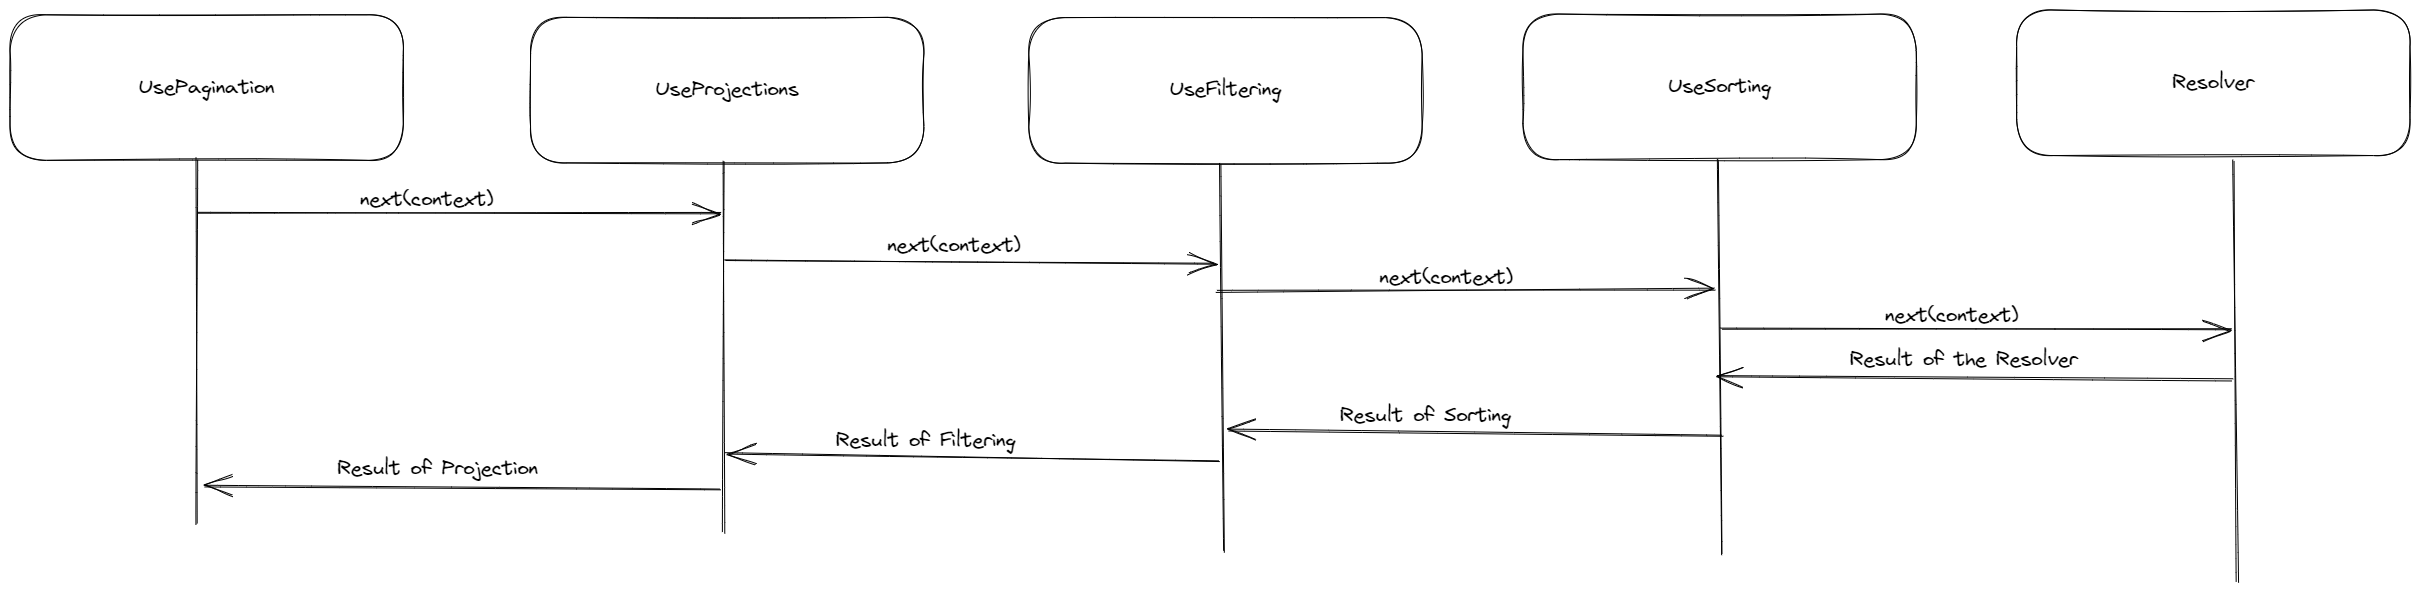
\includegraphics[width=\textwidth]{pics/middleware.png}
    \caption{Exekutierungsreihenfolge Middleware}
\end{figure}

In der obigen Abbildung ist zu sehen, dass die Middleware in der Reihenfolge ausgeführt wird in der sie definiert wurde.
Aber das Resultat welches von der letzten Middleware (dem Resolver) generiert wurde, wird in der umgekehrten Reihenfolge zurückgereicht.
Dabei wird das vom Resolver zurückgelieferte \textit{IQueryable} um die jeweiligen Operationen der restlichen Middleware erweitert.
In den folgenden Abschnitten wird auf die verwendeten Middlewarekomponenten genauer eingegangen: 

\myparagraph{Authorize}
Hierbei wird deklariert, dass nur angemeldete Benutzer Zugriff auf diese Query haben.
Diese Middleware, ist wie in der obigen Schemadefinition ersichtlich, vor dem Resolver auszuführen.
Sie stellt damit sicher, dass nur Anfragen mit einer gültigen Authentifizierung ausgeführt werden.
Im Schema wird das Feld \textit{authors} der Query mit der Direktive \textit{@authorize} versehen.
Näheres zur Authentifizierung und Autorisierung ist im gleichnamigen Abschnitt ersichtlich.

\myparagraph{Projection}
Mit \textit{Projections} liefert HotChocolate die Möglichkeit Over und Underfetching zu verhindern.
Over und Underfetching zu verhindern bedeutet, dass genau jene Daten, welche vom Client angefordert werden, in der Datenbank selektiert und anschließend an den Client zurückgeliefert werden.
Dabei bekommt HotChocolate vom \textit{Resolver} ein \textit{IQueryable}.
Dieses \textit{IQueryable} beinhaltet zunächst nur jene Filterungen und Selektionen welche von der Geschäftslogik festgelegt worden sind.
HotChocolate erweitert dieses \textit{IQueryable} nun durch jene Felder welche in der Query angefordert wurden.

\myparagraph{Filtering}
Aktiviert man die \textit{Filtering} Middleware für ein Query-Field so kann man den implizit von HotChocolate bereitgestellten Sortier-Input verwenden.
Diese Middleware erweitert das vom Resolver zurückgelieferte \textit{IQueryable} um die gegebene Filterung und liefert das Ergebnis der vorangestellten Middleware zurück.
Weiters ist es möglich benutzerdefinierte Typen für die Filterung zu definieren.

\myparagraph{Sorting}
Aktiviert man die \textit{Sorting} Middleware für ein Query-Field so kann man den implizit von HotChocolate bereitgestellten Filter-Input verwenden.
Diese Middleware fügt der vom Resolver zurückgelieferten \textit{IQueryable} die gegebene Sortierung hinzu.
Das Ergebnis wird wiederum an die vorangestellte Middleware zurückgeliefert.
Weiters ist es möglich benutzerdefinierte Typen für die Sortierung zu definieren.

\myparagraph{Zusammenführung Middleware}
Nachdem jene Middleware, welche als erstes definiert wurde, das Ergebnis der restlichen Middlewarekomponenten erhalten hat wird das \textit{IQueryable} ausgeführt und das Ergebnis an den Client zurückgeliefert.

\myparagraph{Ausführung Query und Ergebnis}
\begin{figure}[H]
    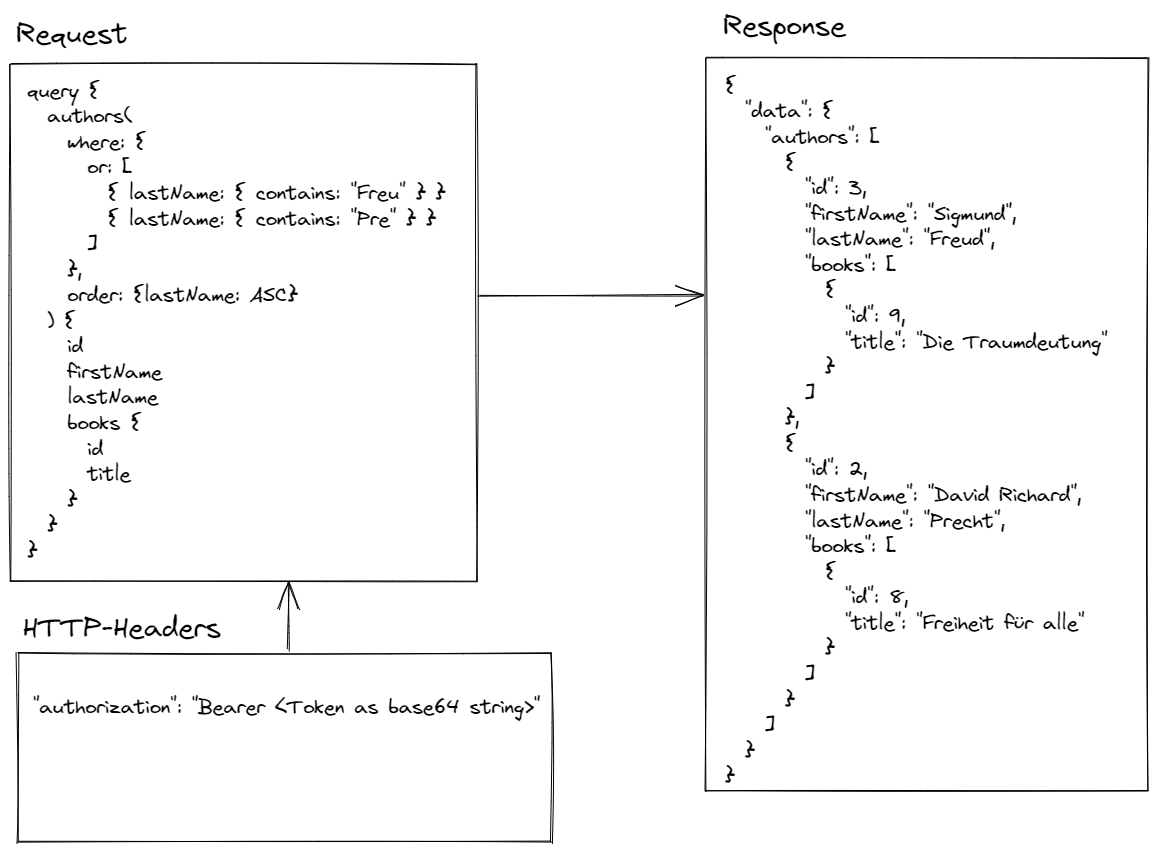
\includegraphics[width=\textwidth]{pics/authors_request.png}
    \caption{Exekutierungsreihenfolge Middleware}
\end{figure}

Die obige Abbildung zeigt eine Query welche alle Autoren mittels dem Feld \textit{authors} abfrägt.
Dabei sollen nur jene Autoren zurückgegeben werden deren Nachname entweder "Freu" oder "Pre" enthält.
Weiters werden die Autoren nach ihrem Nachnamen sortiert.
Bei der Antwort des GraphQL-Service ist zu sehen, dass dieser die Daten genau in jenem Format zurückgibt in dem sie angefragt worden sind.
Mittles HTTP-Parametern wurde der für die Authentifizierung notwendige \textit{JWT-Token} mitübermittelt.
\newline

Die oben abgebildete Anfrage hat am Server folgende Abfrage an die Datenbank ausgelöst:
\begin{JsCode}
SELECT [a].[Id], [a].[FirstName], [a].[LastName], [t].[Id], [t].[Title], [t].[AuthorsId], [t].[BooksId]
FROM [Authors] AS [a]
LEFT JOIN (
    SELECT [b].[Id], [b].[Title], [a0].[AuthorsId], [a0].[BooksId]
    FROM [AuthorBook] AS [a0]
    INNER JOIN [Books] AS [b] ON [a0].[BooksId] = [b].[Id]
) AS [t] ON [a].[Id] = [t].[AuthorsId]
WHERE ((@__p_0 LIKE N'') OR (CHARINDEX(@__p_0, [a].[LastName]) > 0)) OR ((@__p_1 LIKE N'') OR (CHARINDEX(@__p_1, [a].[LastName]) > 0))
ORDER BY [a].[LastName], [a].[Id], [t].[AuthorsId], [t].[BooksId]
\end{JsCode}

\section{Mutations}
Mutations werden wie bereits erwähnt für schreibende Zugriffe auf den GraphQL-Service verwendet.
In den folgenden Abschnitten wird die Umsetzung einer Mutation für das Bearbeiten eines bereits bestehenden Buches erläutert.
Dabei wird auf das Generieren des Schemas zur Laufzeit, als auch der Zugriff auf die Datenbank mittels der Geschäftslogik erläutert.

\myparagraph{Generierung Schema}
Damit ein Client die Möglichkeit hat auf eine Mutation zuzugreifen, muss der Wurzeloperation im Schema das gewünschte Feld hinzugefügt werden.
Dabei wird, wie bereits bei der Implementierung der Query, die Pure-Code-First Vorgehensweise angewandt.
\newline
Im folgenden Code wird die Wurzeloperation Mutation um ein Feld \textit{updateBook} erweitert.
Dabei werden nur Benutzern mit den Rollen Admin oder Bibliothekar die Ausführung gestattet.
Als Übergabeparameter bekommt die Funktion das \textit{DTO BookUpateInput}.
Der Resolver \textit{BookResolver} kümmert sich dabei um Ausführung der Operation.

\begin{JsCode}
public class BookMutation: ObjectTypeExtension<Mutation>{
    protected override void Configure(IObjectTypeDescriptor<Mutation> descriptor) {
        descriptor.Field("updateBook")
            .Authorize(new [] {"Admin", "Librarian"})
            .Argument("input", a => a.Type<NonNullType<BookUpdateInput>>())
            .ResolveWith<BookResolver>(r => r.UpdateBook(default, default))
            .Type<BookType>();
    }
}
\end{JsCode}

Der obige Code resultiert in folgendem Schema:
\begin{JsCode}
type mutation{
    updateBook(input: BookUpdateInput!): Book @authorize(roles: [ "Admin", "Librarian" ], apply: BEFORE_RESOLVER)
}

type Book {
  title: String!
  authors: [Author!]!
  reviews: [Review!]!
  id: Int!
}

type Author {
  firstName: String!
  lastName: String!
  books: [Book!]!
  id: Int!
}

type Review {
  userId: Int!
  user: User!
  bookId: Int!
  book: Book!
  rating: Int!
  id: Int!
}

type User {
  firstName: String!
  lastName: String!
  email: String!
  roles: [Role!]!
  reviews: [Review!]!
  id: Int!
}

type Role {
  name: String!
  users: [User!]!
  id: Int!
}

input BookUpdateInput {
  authors: [Int!]
  id: Int!
  title: String!
}
\end{JsCode}

In dem generierten Schema ist zu erkennen, dass der Objekt-Typ Buch alle Objekt-Typen die dieser explizit oder implizit referenziert, generiert wurden.
Desweiteren wurde die Wurzeloperation Mutation durch das Feld \textit{updateBook} erweitert.
Dieses Feld hat eine \textit{@authorize} Direktive, welche nur Benutzern mit den Rollen Admin oder Bibliothekar Zugriff gewährt.
Weiters wurde das Input-Objekt \textit{BookUpdateInput} generiert.
\newline

Das Input-Objekt \textit{BookUpateInput} wurde dabei zusätzlich wie folgt deklariert:
\begin{JsCode}
public class BookUpdateInput: InputObjectType<BookUpdate> {

    protected override void Configure(IInputObjectTypeDescriptor<BookUpdate> descriptor) {
        descriptor.Field(f => f.Authors).Type<ListType<NonNullType<IntType>>>();
    }
}

public class BookUpdate {
    public int Id { get; set; }
    public string Title { get; set; }
    public ICollection<int> Authors { get; set; }
}
\end{JsCode}

Bei der Definition des Input-Objekts \textit{BookUpdateInput} bietet die \textit{Configure} Methode der Basisklasse \textit{ObjectType} wiederum die Möglichkeit genauere Definitionen vorzunehmen.
Im obigen Code-Beispiel ist ersichtlich, dass das Feld \textit{Authors} eine Liste von \textit{Integer} enthält die nicht \textit{null} sein dürfen.
\newline

Anders als die im Datenbankschema beschriebene Entität Buch, hält das Input-Objekt \textit{BookUdpateInput} keine Liste des Objekt-Typs Autor, sondern nur eine Liste von \textit{Integer} Werten, welche die IDs wiederspiegeln.
Mit dieser Vorgehensweise wird einer zyklischen Abhängigkeit vorgebeugt, denn sonst würden die Bücher Autoren referenzieren, welche wiederum Bücher referenzieren und das wiederholt sich endlos.
Um diese \textit{DTOs} wieder zu Domänenklassen umzuwandeln müssen sie gemappt werden.
Dafür wird im Prototypen \textit{AutoMapper} verwendet.

Im folgenden Code-Beispiel wird \textit{BookUpdateInput} wieder zu \textit{Book} umgewandelt:
\begin{JsCode}
public class BookProfile : Profile {
    public BookProfile() {
        CreateMap<BookUpdate, Book>()
            .ForMember(
            dest => dest.Authors,
            opt => opt.MapFrom(src => src.Authors.Select(id => new Author { Id = id })));
    }

}
\end{JsCode}

Zum Vergleich hier noch die Klasse \textit{Book} welche das Domänenobjekt Buch darstellt und von \textit{BaseEntity} ableitet und damit eine \textit{Id} erbt.

\begin{JsCode}
public class Book: BaseEntity {
    public string Title { get; set; }
    public List<Author> Authors { get; set; } = new List<Author>();
    public List<Review> Reviews { get; set; } = new List<Review>();
}
\end{JsCode}

\myparagraph{Ausführung und Ergebnis}

\begin{figure}[H]
    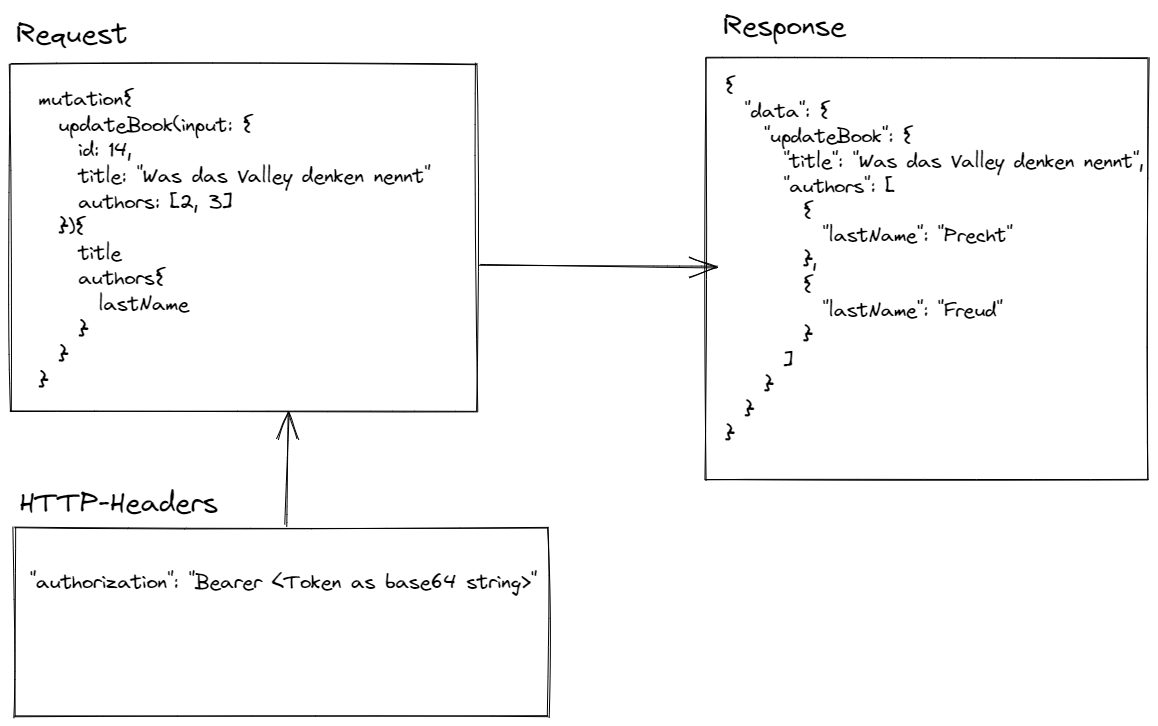
\includegraphics[width=\textwidth]{pics/execution_mutation.png}
    \caption{Schemadefinition}
\end{figure}

In dieser Abbildung ist die Ausführung des Feldes \textit{updateBook} der Mutation zu sehen.
Der Anfrage muss als HTTP-Header ein \textit{JWT-Token} übergeben werden um zu überprüfen ob der ausführende Benutzer genügend Rechte hat.
Die Antwort des GraphQL-Service entspricht dabei wiederum genau dem Schema welches in der Query der Anfrage angegeben wurde.


\section{Subscriptions}
Subscriptions werden wie bereits erwähnt, verwendet um bidirektionale Kommunikation zwischen dem Client und Server zu ermöglichen.
Dabei registriert sich der Client auf Events welche vom Server ausgelöst werden und bekommt dadurch in Echtzeit Updates.
HotChocolate realisiert Subscriptions mittels WebSockets.
HotChocolate bietet dabei 2 Subscription Provider: \textit{In-Memory} und \textit{Redis}.
Für den Prototypen wurde dabei die \textit{In-Memory} Version verwendet.

\myparagraph{Subscription über Event benachrichtigen}
Um eine Subscription über ein ausgeführtes Event zu benachrichtigen stellt HotChocolate den \textit{ITopicEventSender} und den \textit{ITopicEventReceiver} zur Verfügung.
Diese Interfaces sind Abstraktionen der Funktionalitäten des Subscription Providers.
Diese Abstraktion ermöglicht es dem Entwickler den Subscription Provider je nach Bedarf zu einem späteren Zeitpunkt beliebig auszutauschen.
Um nun eine Subscription von zu benachrichtigen ist folgender Code notwendig:
\begin{JsCode}
public async Task<Book> CreateBook([Service] IBookService bookService, BookCreate input,[Service] ITopicEventSender sender) {
    var book = await bookService.AddAsync(mapper.Map<Book>(input));
    await sender.SendAsync("bookAdded", book);
    return book;
}
\end{JsCode}

In Zeile 3 des obigen Code-Beispiels wird mittels dem \textit{ITopicEventSender} der \textit{ITopicEventReceiver} von dem neu erstelltem Buch notifiziert.
Auf die Verwendung des \textit{ITopicEventReceiver} wird in der folgenden Erläuterung der Implementierung einer Subscription, welche auf die Erstellung eines Buches wartet, näher eingegangen:

\myparagraph{Schemagenerierung}
Für die Generierung des Schemas wird die Pure-Code-First Methode von GraphQL verwendet.
Die Wurzeloperationen Subscription wird dabei um ein Feld \textit{bookAdded} erweitert.
Die Umsetzung ist dabei in folgendem Code-Beispiel ersichtlich:

\begin{JsCode}
public class BookSubscription: ObjectTypeExtension<Subscription> {
    protected override void Configure(IObjectTypeDescriptor<Subscription> descriptor) {
        descriptor
        .Field("bookAdded")
        .Type<BookType>()
        .Resolve(context => context.GetEventMessage<Book>())
        .Subscribe(async context => {
            var receiver = context.Service<ITopicEventReceiver>();
            return await receiver.SubscribeAsync<string, Book>("bookAdded");
        });
    }
}    
\end{JsCode}
In Zeile 9 des obigen Code-Beispiels ist ersichtlich, dass der \textit{ITopicEventReceiver} auf eine Benachrichtigung durch den \textit{ITopicEventSender} wartet.

Der oben stehende Code generiert dabei folgendes Schema:
\begin{JsCode}
type subscription{
    bookAdded: Book
}

type Book {
  title: String!
  authors: [Author!]!
  reviews: [Review!]!
  id: Int!
}

type Author {
  firstName: String!
  lastName: String!
  books: [Book!]!
  id: Int!
}

type Review {
  userId: Int!
  user: User!
  bookId: Int!
  book: Book!
  rating: Int!
  id: Int!
}

type User {
  firstName: String!
  lastName: String!
  email: String!
  roles: [Role!]!
  reviews: [Review!]!
  id: Int!
}

type Role {
  name: String!
  users: [User!]!
  id: Int!
}
\end{JsCode} 

\myparagraph{Ausführung und Ergebnis}


\section{Authentifizierung und Autorisierung}
Authentifizierung ist der Vorgang mit dem die Identität eines Benutzers festgestellt wird.
Die Autorisierung wiederum ermittelt ob ein Benutzer die erforderlichen Rechte hat, um auf eine bestimmte Ressource hat.
Wie im Anwendungsszenario bereits beschrieben, gibt es im System 3 Rollen für Benutzer: User, Librarian und Admin.
Jede Rolle kann dabei nur für Sie freigegebene Ressourcen zugreifen.
\newline

Die Authentifizierung und Autorisierung für den Prototypen wird mit \textit{JWT-Tokens} und der Zuhilfenahme der \textit{ASP.NET Core-Authentifizierung} umgesetzt.
Die folgenden Abbildungen beschreiben die Rollen und die Ressourcen auf die sie Zugriff haben.
Grüne Felder bedeuten dabei, dass auch Benutzer ohne valides \textit{JWT-Token} Zugriff auf diese Ressource haben.
Das gelbe Feld "Einloggen" kann nur nach einer bereits erfolgten Registrierung aufgerufen werden.
Rote Felder wiederum verlangen ein valides \textit{JWT-Token} und sind an die Rolle des aufrufenden Benutzers gebunden.

\begin{figure}[H]
    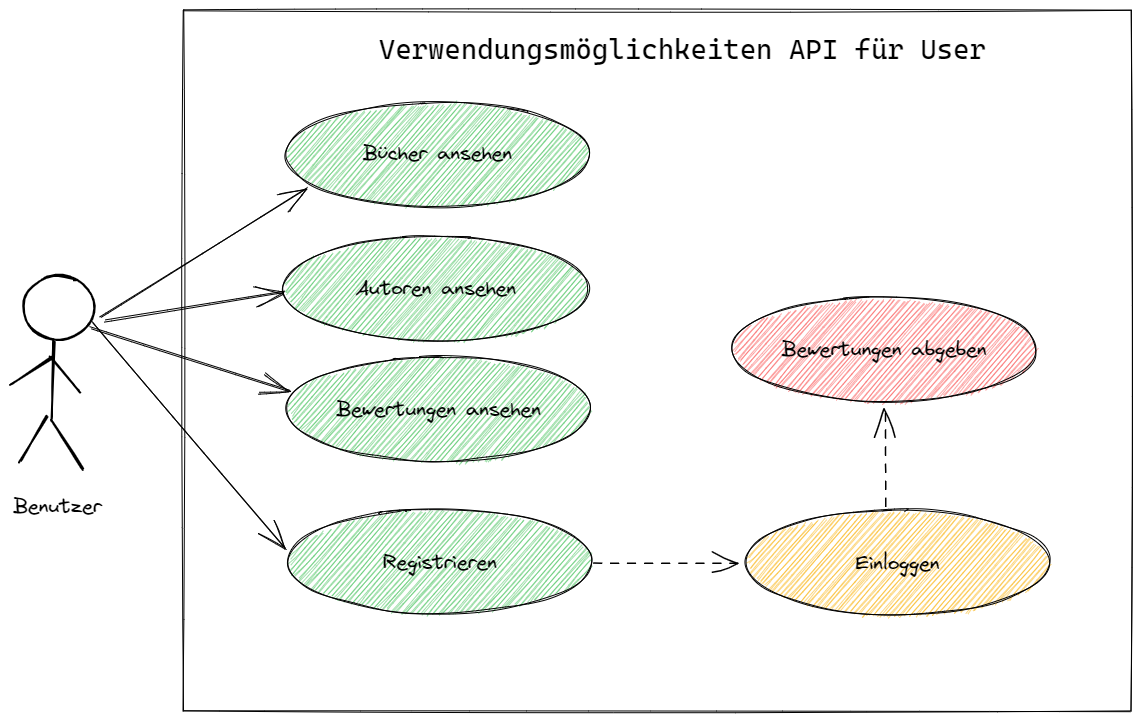
\includegraphics[width=\textwidth]{pics/UseCaseUser.png}
    \caption{Rechte User.}
\end{figure}

\begin{figure}[H]
    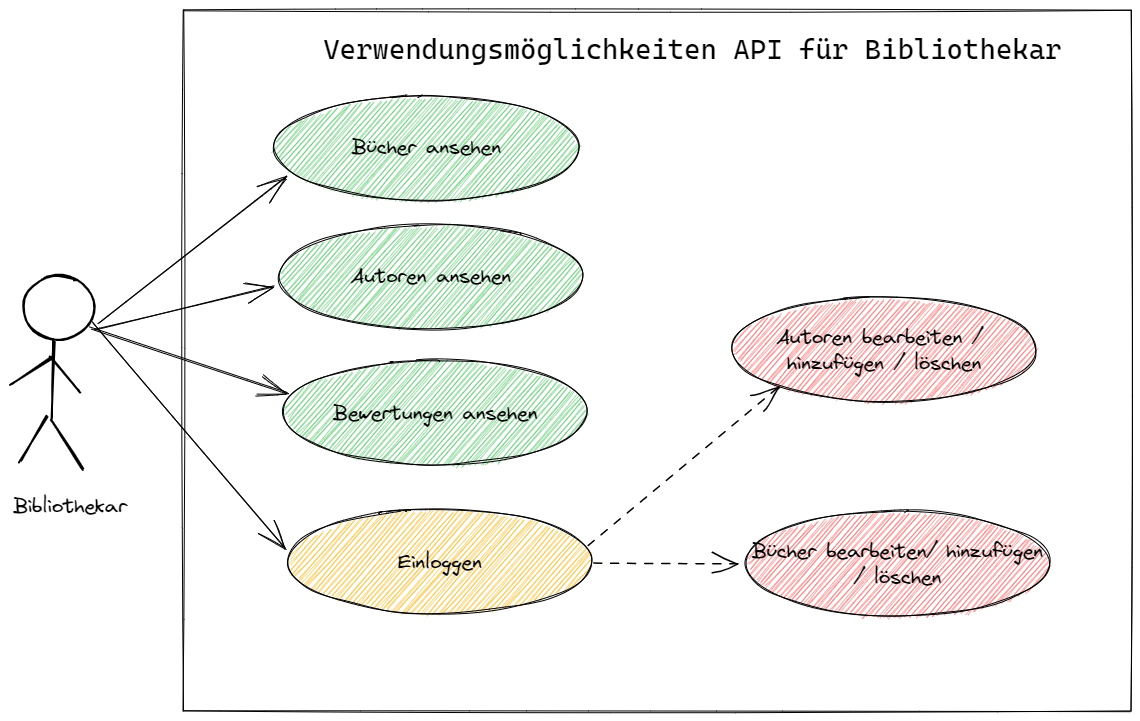
\includegraphics[width=\textwidth]{pics/UseCaseLibrarian.png}
    \caption{Rechte Bibliothekar.}
\end{figure}

\begin{figure}[H]
    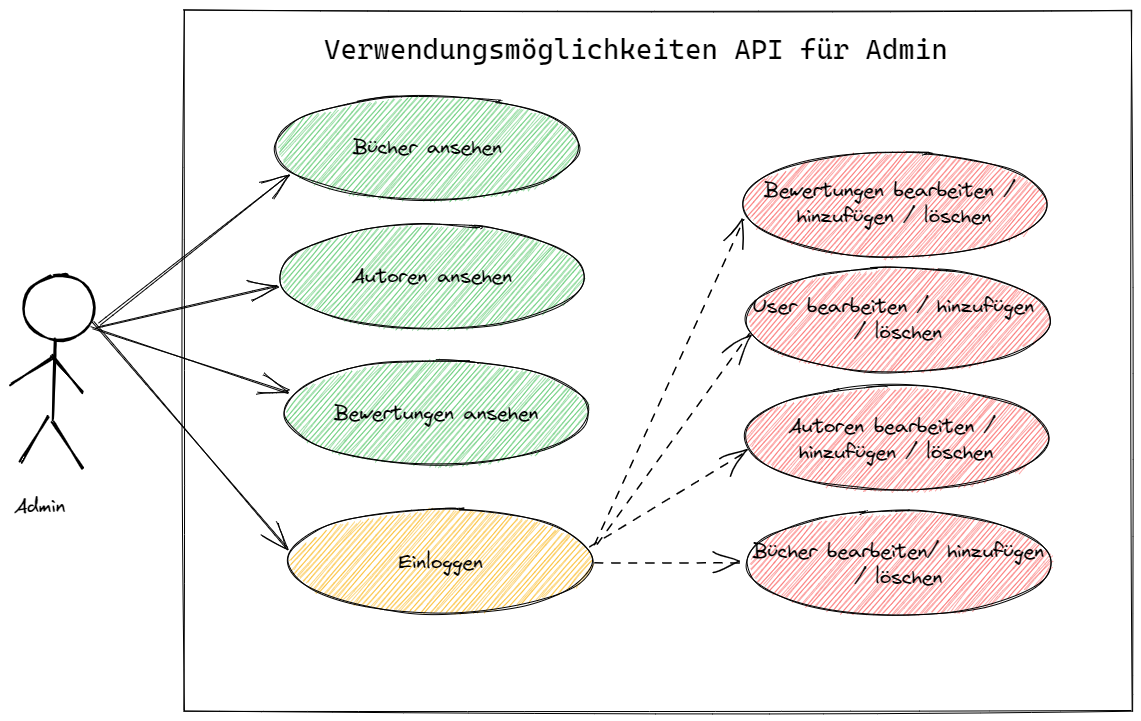
\includegraphics[width=\textwidth]{pics/UseCaseAdmin.png}
    \caption{Rechte Admin.}
\end{figure}

\myparagraph{Generierung JWT-Token}
Um die Authentifizierung mittels JWT-Token zu ermöglichen muss diese Authentifizierungsform erst registriert werden.
Diese Registrierung erfolgt, wie in .NET üblich, im \textit{WebApplicationBuilder}.

\begin{JsCode}
builder.Services.AddAuthentication(JwtBearerDefaults.AuthenticationScheme)
    .AddJwtBearer(options => {
        var tokenSettings = configuration
        .GetSection("JWT").Get<TokenSettings>();
        options.TokenValidationParameters = new TokenValidationParameters {
            ValidIssuer = tokenSettings.Issuer,
            ValidateIssuer = true,
            ValidAudience = tokenSettings.Audience,
            ValidateAudience = true,
            IssuerSigningKey = new SymmetricSecurityKey(Encoding.UTF8.GetBytes(tokenSettings.Key)),
            ValidateIssuerSigningKey = true
        };
    });
\end{JsCode}

Im obigen Code ist zu sehen, dass dem Server auf dem der GraphQL-Service läuft, eine JWT-Token Authentifizierung hinzugefügt wird.
Hierzu wurde eine Klasse \textit{TokenSettings} erstellt welche den \textit{Issuer}, die \textit{Audience} und den \textit{Key} welche die benötigten Daten aus der \textit{appsettings.json} liest und bereitstellt.
\newline

Nachdem die zu verwendende Authentifizierungsmethode am Server registriert ist, ist es notwendig die Logik für die Erstellung eines Tokens zu implementieren.
Diese wurde im \textit{AuthService} in der Methode \textit{Login} umgesetzt.
Diese Methode erhält dabei einen Benutzernamen und ein Passwort als Übergabeparameter.
Hervorzuheben ist dabei, dass der Login als Mutation umgesetzt wurde.
Zum jetzigen Zeitpunkt finden zwar keine schreibenden Operationen in dieser Methode statt, aber Login-Operationen beinhalten beispielsweise oftmals das Speichern des Letzten erfolgreichen Logins.
\newline

Im folgenden Code-Beispiel wird ein JWT-Token, bei übereinstimmenden User-Credentials, generiert.

\begin{JsCode}
public async Task<string> Login(string email, string password) {

    var user = await userRepository.GetFirstAsync(user => user.Email.Equals(email), user => user.Roles);
    if (user is not null && BCrypt.Net.BCrypt.Verify(password, user.Password)) {
        var securtityKey = new SymmetricSecurityKey(Encoding.UTF8.GetBytes(tokenSettings.Key));

        var credentials = new SigningCredentials(securtityKey, SecurityAlgorithms.HmacSha256);

        var claims = new List<Claim>();

        claims.Add(new Claim("FirstName", user.FirstName));
        claims.Add(new Claim("LastName", user.LastName));
        claims.Add(new Claim("Email", user.Email));
        if (user.Roles?.Count > 0) {
            foreach (var role in user.Roles) {
                claims.Add(new Claim(ClaimTypes.Role, role.Name));
            }
        }

        var jwtSecurityToken = new JwtSecurityToken(
            issuer: tokenSettings.Issuer,
            audience: tokenSettings.Audience,
            //expires: DateTime.Now.AddMinutes(30),
            expires: DateTime.Now.AddDays(1),
            signingCredentials: credentials,
            claims: claims
        );

        return new JwtSecurityTokenHandler().WriteToken(jwtSecurityToken);
    }

    return "";
}
\end{JsCode}

Der obige Code beinhaltet die Überprüfung der vom Client übergebenen Benutzerdaten.
Stimmen diese mit jenen in der Datenbank überein, so wird ein JWT-Token generiert.
Der Token beinhaltet dabei folgende Daten des Benutzers: Vorname, Nachname, Email und die zugewiesenen Rollen.

\myparagraph{Verwendung Authentifizierung und Autorisierung}
Um ein Feld einer Query, Mutation oder Subscription nun abzusichern muss man die Field-Middleware Authentifizierung bei dem jeweiligen Feld aktivieren.
% Mit Pure-Code-First funktioniert das wie im folgenden Code-Beispiel abgebildet:
Mit der Pure-Code-First Methode von HotChocolate wird die Konfiguration in der \textit{Configure} Methode des jeweiligen \textit{ObjectType} abgebildet.

\begin{JsCode}
public class AuthorQuery: ObjectType<Query> {
    protected override void Configure(IObjectTypeDescriptor<Query> descriptor) {
        descriptor.Field("authors")
            .ResolveWith<AuthorResolver>(r => r.Authors())
            .Authorize()
            .Type<ListType<NonNullType<AuthorType>>>();
    }
}
\end{JsCode}

In dem oben stehenden Code wird festgelegt, dass ein User ein valides \textit{JWT-Token} an de Service übergeben muss um Zugriff auf die Ressource zu haben.
Im Umkehrschluss bedeutet dies, dass jeder Benutzer des Systems, wenn er angemeldet ist, Zugriff auf diese Ressource hat.
\newline

\begin{JsCode}
public class AuthorQuery: ObjectType<Query> {
    protected override void Configure(IObjectTypeDescriptor<Query> descriptor) {
        descriptor.Field("authors")
            .ResolveWith<AuthorResolver>(r => r.Authors())
            .Authorize(new [] {"Admin", "Librarian"})
            .Type<ListType<NonNullType<AuthorType>>>();
    }
}
\end{JsCode}
Dieser Code erweitert die erste Version um Autorisierung.
Es haben somit nur mehr Benutzer mit den Rollen Admin und Bibliothekar Zugriff auf diese Ressource.
Ein "normaler" Benutzer würde abgewiesen werden.

\section{1 + n Problem}
Lösung mit Dataloader




\chapter{Conclusio}

\section{Fazit}

\section{Ausblick}

\bibliography{literatur}


\end{document}
